\documentclass[12 pt, a4paper, toc=graduated, oneside]{book}
\usepackage{amsmath, amssymb,amsfonts, amsthm, mathtools}
\usepackage[utf8]{inputenc}
\usepackage{pifont}
\usepackage[inline]{enumitem}
\usepackage{graphicx}
\usepackage{cancel}
\usepackage{soul}
\usepackage{tikz-cd}
\usepackage{tikz}
\usetikzlibrary{calc,trees,positioning,arrows,fit,shapes,calc}

\setlength\parindent{0pt}

\usepackage{geometry}
 \geometry{
 a4paper,
 total={170mm,257mm},
 left=20mm,
 top=20mm,
 }
 
\usepackage{fancyhdr}
\usepackage[english]{babel}

\pagestyle{fancy}
\fancyhf{}
\rfoot{Page \thepage}
\renewcommand{\footrulewidth}{1pt}
\fancypagestyle{plain}{%
\fancyhf{}% clears all header and footer fields
\rfoot{Page \thepage}}

\usepackage{titlesec}
\titleformat{\chapter}[block]
  {\normalfont\huge\bfseries}{}{0 em}{\Huge}
\titleformat{\section}[block]
  {\normalfont\Large\bfseries}{\thesection}{1em}{\Large}
\titlespacing*{\chapter}{0pt}{-19pt}{0pt}

\usepackage{chngcntr}
\counterwithin{footnote}{chapter}

\newcommand{\pah}[1]{\rhead{Prof. A. Hariharan}
    #1
    \begin{flushright}
    -Professor Ananthnarayan Hariharan\\
    \hrulefill\\
    \end{flushright}}
\newcommand{\prs}[1]{\rhead{Prof. R. Santhanam}
    #1
    \begin{flushright}
    -Professor Rekha Santhanam\\
    \hrulefill\\
    \end{flushright}}
\newcommand{\assign}[1]{\rhead{Assignment}
    #1
    
    \hrulefill\\}
\newcommand{\example}[1]{\refstepcounter{example}\par\medskip
   {\color{examplecolor}{\textbf{Eg~\thechapter.\theexample. }#1}} \rmfamily}
\newcommand{\highlight}[1]{{\color{highlightcolor}{#1}}}
\newcommand{\exercise}[1]{\refstepcounter{exercise}\par\medskip
   {\color{exercisecolor}{\textbf{Ex~\thechapter.\theexercise. }#1}} \rmfamily}
\newcommand{\xmark}{\ding{55}}
\newcommand{\LoT}{\hyperref[sec:LoT]{Law of Trichotomy}}
\newcommand{\simpleexample}[1]{{\color{examplecolor}{#1}}}
\newcommand{\claim}[2]{{\color{claimcolor}{%
            \textbf{Claim: }#1\\%
            \textbf{\textit{Proof}: }#2}} \\}
\newcommand{\axiom}[1]{\refstepcounter{axiom}\par\medskip
   \label{ax:A\theaxiom}\textbf{A\theaxiom. }%
   \begin{tabular}[t]{l}
        #1 
   \end{tabular}%
   \rmfamily}
\newcommand{\refaxiom}[1]{\hyperref[ax:A#1]{A#1}}
\newcommand{\lub}{\operatorname{lub}} 
\newcommand{\glb}{\operatorname{glb}} 
\newcommand{\floor}[1]{\lfloor #1 \rfloor}
 
\newcounter{exercise}[chapter]
\newcounter{example}[chapter]
\newcounter{axiom}
%\newenvironment{exercise}[1][]{}{\medskip}

\usepackage[dvipsnames]{xcolor}
\definecolor{mylinkcolor}{RGB}{00,00,75}
\definecolor{examplecolor}{RGB}{00, 75, 00}
\definecolor{highlightcolor}{RGB}{75, 00, 00}
\definecolor{exercisecolor}{RGB}{81, 40, 00}
\definecolor{claimcolor}{RGB}{29, 100, 100}

\usepackage{hyperref}
\hypersetup{
    colorlinks=true,
    linkcolor=mylinkcolor,
    filecolor=magenta,      
    urlcolor=cyan,
%    bookmarks=true,
}
\title{MA 107}
\author{Aryaman Maithani}
\date{}

\begin{document}
\frontmatter
\maketitle
\tableofcontents
%\addtocontents{toc}{~\hfill\textbf{Page}\par}
\newpage
\chapter{Introduction}
\iffalse Proper introduction to be finalised at the end, main points:
\begin{enumerate}
    \itemsep0em
    \item Not a formal book, supposed to be notes.
    \item Every chapter corresponds to a different lecture.
    \item Two topics were taught parallel-y. The beginning of every chapter mentions which professor has taught that so that the reader knows the flow. (The name of the professor is mentioned in the header of every following page of that chapter as well.)
    \item As the classes sort of complement each other, do read them in chronological order.
    \item {\color{mylinkcolor}{Text written in this shade of blue represents a hyperlink (except for this text itself) and depending on your file viewer, you can click on it to jump to the appropriate section. (Do note your position before clicking on it, though.)}}
    \item There are other colours also used in this document which you would understand yourself after you start reading.
    \item Appreciate the course!
\end{enumerate}
\fi
Hello, if you're reading these notes, you are most likely a BS Math student.\\
These are the notes that I made when I was taking this course in Spring 2019. I hope that you find them helpful and clear.\\
Here are some things that I'd like to point out
\begin{enumerate}[nosep] 
	\item This not meant to be a substitute for a formal book, these are just notes. However, I have tried to write them in as consistent and formal a way as possible. As you'd see, the nature of the course makes it a bit difficult to do so as it's somewhat a course on \emph{How to think Mathematically.}
    \item Every chapter corresponds to a different lecture.
    \item Two topics were taught parallel-y. The beginning of every chapter mentions which professor has taught that so that the reader knows the flow. (The name of the professor is mentioned in the header of every following page of that chapter as well.)
    \item As the classes sort of complement each other, do read them in chronological order.
    \item {\color{mylinkcolor}{Text written in this shade of blue represents a hyperlink (except for this text itself) and depending on your file viewer, you can click on it to jump to the appropriate section. (Do note your position before clicking on it, though.)}}
    \item There are other colours also used in this document which you would understand yourself after you start reading.
\end{enumerate}
Lastly, take this course with an open mind and appreciate the rigour and formalism to which you'll be introduced.\\
You might often come across topics which just seem very \emph{absurd} to prove. However, you must take a step back to see what is it really that you're proving.\\\\
As an example, you'll prove $1 > 0$ at some point of time. This is also the point of time that many lose their minds and feel like this may have been a wrong choice of major. However, what you're \emph{really} proving is that the \emph{multiplicative identity} is greater than the \emph{additive identity.} If you take one more step back, you'll also see that being ``greater'' just means that $1$ is related to $0$ in a certain manner such that the relation follows some certain axioms.\\
Once you realise that `$1$', `$0$' and `$>$' are just some arbitrary symbols which follow certain rules, it would (hopefully) feel less absurd that you actually \emph{need} to prove $1 > 0,$ you might even \emph{appreciate} that this is something that can indeed be proven.\\
Most likely, you'll also prove a result along the way using which you can also show that $\mathbb{C}$ can never be given a ``nice enough'' order. How neat is that?

\hrulefill

These notes are also supplemented with the assignments that were given; which have been placed at the appropriate location. It would be nice practice to solve the assignments alongside.
%
\mainmatter
\lhead{MA 107: Lecture \thechapter}
\chapter{Lecture 1}
\pah{03-01-2019}
\section{Mathematical statements}\label{sec:state}
What is a mathematical statement?\\
Is there any \textit{real} definition of a mathematical statement or is every sentence a mathematical statement?\\
Here are some sentences:
\begin{enumerate}
    \itemsep0em
    \item 2 is an even prime.
    \item Chirag is a good man.
    \item 5 is an even number.
    \item The sky is blue.
    \item There are chairs and tables in LT 101.
    \item I love Mathematics.
    \item Euler was smart.
\end{enumerate}
Are all of the above mathematical statements? The answer is: no.\\
2, 6 and 7 are not mathematical statements.\\
It might have become a bit clearer as to what a mathematical statement is. Do notice that 3 \textbf{\textit{is}} in fact, a mathematical statement.\\
Furthermore, we might not know right away whether there are chairs and tables in LT 101 but what we \textbf{\textit{do}} know is that that sentence would be either true or false.\\

Simply put, \highlight{a mathematical statement is a sentence which is either true or false.}\\

Now, if see the problem with the 2, 3 and 7. It is the fact that ``good", ``love" and ``smart" aren't properly defined. What might be good for Chirag might not be what is good for me, et cetera. So, while most \textit{might} agree that Euler was smart, it is \textbf{\textit{not}} a mathematical statement.\\
In Mathematics, we always phrase things in statements which do have a definite truth value.\footnote{\label{ft:conjec} We have things in Mathematics known as \textit{conjectures} which are unproven \textbf{statements}. So, even though \textit{we} do not know their truth value, they \textit{do} have a \textit{definite} truth value.}\\
We are also precise when we state things.\\
\newpage
%
%
%
\subsection{Compound Statements}\label{ssec:compound}
If we look at the 5$^{\text{th}}$ sentence above which we decided to call a statement, we can see that it is more ``complicated". For that statement to be true, it demands \textbf{\textit{two}} things to be true, namely:
\begin{enumerate}
    \itemsep0em
    \item There must be chairs in LT 101.
    \item There must be tables in LT 101.
\end{enumerate}
On the other hand, consider the statement: ``There are chairs \textit{or} tables in LT 101.". For this statement to be true, it just demands that at least \textbf{\textit{one}} of the above two be true. (Both may also be true.)\\~\\
The symbol for ``and" is ``$\land$".%
\footnote{to help remember: $\land$ looks like an `A' which stands for ``and"}%
The symbol for ``or" is ``$\lor$".\\~\\
So, finally, if p and q are two statements, then:
\begin{enumerate}[label = C\arabic*.]
    \itemsep0em
    \item \label{comp1}(p $\land$ q) is true if and only if \textbf{both} p and q are true.
    \item \label{comp2}(p $\lor$ q) is true if and only if \textbf{at least} one of p or q is true.
\end{enumerate}
%
%
%
\subsection{Negation}\label{ssec:neg}
When given a statement, it often helps to look at its negation%
\footnote{\label{ft:neg} technically, we haven't defined \textit{what} a negation is. It is assumed that you do know what it is. In case you don't (or that you want to be formal), you may take the ``property" mentioned above as the definition.}%
\ 
as they have exactly opposite truth values. In other words, given a statement and its negation, \textit{exactly} one of them is true.\\

The easiest way to negate a statement is to place a ``not" in the statement. (At the appropriate location.)\\
\example{%
Statement: x is an even number.\\
Negation: x is \textit{not} an even number.}\\
Even though you might be tempted to say \simpleexample{``x is an odd number"} as the negation, it is not correct.\\
Why? Simply because we do not know what x is. $\frac{1}{2}$, for example, is neither even nor odd.\\
Had we known that x \textit{is} an integer, then it would have been correct to say that the negation is \simpleexample{``x is an odd number"}.\\

Also, to introduce the notation, the negation of a statement is denoted by placing a `$\sim$' before the statement.\\
\example{S: x is an even number.\\
$\sim$S: x is \textit{not} an even number.}
\\~\\
Now, we'll move on to a slightly more complicated type of statement.\\
Suppose A wants to buy a phone with a 40 MP camera \textit{and} a 4 GB RAM. A goes and buys a phone. When has A \textit{not} bought the originally desired phone?\\
Consider the following table:\\~\\
\begin{tabular}{c|c c}
    Phone Type & 40 MP camera & 4 GB RAM \\
    \hline
    P$_1$ & \checkmark & \checkmark \\
    P$_2$ & \checkmark & \xmark \\
    P$_3$ & \xmark & \checkmark \\
    P$_4$ & \xmark & \xmark \\
\end{tabular}\\
The above table makes it clear that A wants to buy P$_1$. So, if they buy any other type of phone, they have \textit{not} bought it.\\
Therefore, if your answer originally had just been: ``When A has bought a phone which has neither a 40 MP camera nor a 4 GB Ram.", you  can see how that is not complete. You have missed the cases where just one functionality is missing.\\
This reasoning is also consistent with how we defined \hyperref[comp1]{``and"}.\\
So, a concise way to phrase the answer would be: ``A has not bought the desired phone if the phone is \textit{either} missing a 40 MP camera \textit{or} a 4 GB RAM."

\hrulefill
\exercise{Do the same for the condition- ``a 40 MP camera \textit{or} a 4 GB RAM".}

\hrulefill\\
It might now be clear what the relation between ``and" and ``or" is when it comes to negation.
\begin{enumerate}
    \itemsep0em
    \item $\sim(p\land q) \equiv \sim p \lor \sim q$
    \item $\sim(p\lor q) \equiv \sim p \land \sim q$
\end{enumerate}
The ``$\equiv$" symbol used above stands for "is equivalent to". Two statements are said to be equivalent if they have the exact same truth value.\\~\\
Now, let's see another aspect of negation.
\begin{center}
    \example{%
        \begin{tabular}{|c|c}
            Case 1 & Case 2\\
            \hline
            S: $x \in \mathbb{R} \land x > 0$ & Let $x \in \mathbb{R}$ \\
            $\sim$ S: $x \not \in \mathbb{R} \lor x \not > 0$ & S: $x > 0$\\
             & $\sim$ S: $x \not > 0$
        \end{tabular}
    }
\end{center}
The difference between case 1 and case 2 is that in case 2, $x$ is defined to be real number which is \textbf{\textit{not}} going to be negated. In another words, it could be thought of as being part of the ``hypothesis" and being unquestionable.

\hrulefill
\exercise{Let X be a set. Let A and B be subsets of X. Write a statement that means: A is a subset of B.}
\exercise{\label{ex:1.3}$x \in \mathbb{R}$\\
Negate: Given $x > 0$\\
You may have thought of another way of negating that statement apart from $x\not > 0$, can you justify why that works?
}

\hrulefill
%
\chapter{Lecture 2}
\pah{07-01-2019}
Going back to \hyperref[ex:1.3]{Ex 1.3.}, your answer might have been ``x $\le$ 0".\\
The justification of that comes from a property of real numbers, known as the \highlight{Law of Trichotomy}.
\section{Law of Trichotomy}\label{sec:LoT}
Let $x \in \mathbb{R}$. Then \textit{exactly} 1 of the following is true:
\begin{enumerate}
    \itemsep0em 
    \item $x < 0$
    \item $x = 0$
    \item $0 < x$
\end{enumerate}
Note that it was important to use the word \textit{``exactly"}. Had it not been used, it could have been possible that more than one of those statements is true at the same time. Therefore, the law becomes stronger with the addition of the word ``exactly".\\
Now, it is clear why $x \not > 0 \equiv x \le 0$. (Ponder what $x \le 0$ means in terms of $<$ and $=$.)

\hrulefill
\exercise{State \LoT{} in an equivalent way involving any $x, y \in \mathbb{R}$. $\big($To show equivalence, try introducing (x-y).$\big)$}

\hrulefill
\section{Quantifiers}\label{sec:quant}
Let us now try to write some simple statements in a mathematical manner.\\
\example{\label{exam:2.1}
    \begin{tabular}{|r l}
        English: & Every bench is this room is brown. \\
        Math: & Let B = set of benches in this room.\\
              & $\forall b \in B\left(\text{b is brown.}\right)$
    \end{tabular}
}\\
\example{%
    \begin{tabular}{|r l}
        English: & There is a brown bench in this room. \\
        Math: & Let B = set of benches in this room.\\
              & $\exists b \in B\left(\text{b is brown.}\right)$
    \end{tabular}
}\\~\\
As you can see, two new symbols have been introduced. Considering the English statement was written above the mathematical one, you might have an intuition as to what the symbols mean.
%
%
\subsection{The Universal Quantifier \texorpdfstring{$\left(\forall\right)$}{}} \label{ssec:univquant}
$\forall$ is the symbol used when we are talking about \textit{every} element of some set. It is pronounced as ``for all".\\
``$\forall b \in B$" would be read ``for all b belonging to B".\\
For one's own clarity, it may also be inferred as ``given \textit{any} b belonging to B".\\
As you might have understood, it is used when we want to make a statement which applies to \textit{every} element of some set.
%
%
\subsection{The Existential Quantifier \texorpdfstring{$\left(\exists\right)$}{}} \label{ssec:exisquant}
$\exists$ is the symbol when we want to talk about the \textit{existence} of some element with a certain property. It is pronounced as ``there exists a(n)"\\
``$\exists b \in B$" would be read ``there exists a b belonging to B".\\
It is used when we want to make a statement expressing the {\color{blue}{existence}} of {\color{orange}{some element}} in a {\color{red}{set}} for which some {\color{brown}{certain statement}} is true. Example: ${\color{blue}{\exists}} {\color{orange}{b}} \in {\color{red}{B}} \left({\color{brown}{\text{b is brown.}}}\right)$\\
Note that \textbf{existence does not imply uniqueness.}
%
%
\section{Negating Quantifiers}\label{sec:negquant}
The above two quantifiers mentioned perform complementary roles when it comes to negation. To illustrate this, let's go back to the \hyperref[exam:2.1]{Eg. \thechapter.\ref*{exam:2.1}}.
\example{%
\begin{tabular}{|c|c|c|}
    \hline
     & Statement & Negation\\
     \hline
     English: & Every bench is this room is brown. & ?? \\
     \hline
        Math: & Let B = set of benches in this room. & \\
              & $\forall b \in B\left(\text{b is brown.}\right)$ & ??\\
    \hline
\end{tabular}
}\\~\\
Let us first try to think of the negation in English.\\
Is it ``Every bench is this room is \textit{not} brown."?\\
No. It is not. (Why?)\\
Let us try to think when would the original statement be false. You can think of it as ``What would one person have to do to prove the statement wrong?"\\
As the claim is that \textit{every} bench is brown, it would be sufficient to find \textit{any} one bench which is \textit{not} brown.
\addtocounter{example}{-1}
\example{%
\textbf{(contd.)}\\
\begin{tabular}{|c|c|c|}
    \hline
     & Statement & Negation\\
     \hline
     English: & Every bench is this room is brown. & There is \textit{a} bench in this room which is not brown. \\
     \hline
        Math: & Let B = set of benches in this room. & \\
              & $\forall b \in B\left(\text{b is brown.}\right)$ & ??\\
    \hline
\end{tabular}
}\\~\\
It might now be clear as to why the quantifiers play a complementary role. As the English concluded the \textit{existence} of a particular type of bench, it becomes clear that the existential quantifier must be used. This finally completes the example:
\addtocounter{example}{-1}
\example{%
\textbf{(contd.)}\\
\begin{tabular}{|c|c|c|}
    \hline
     & Statement & Negation\\
     \hline
     English: & Every bench is this room is brown. & There is \textit{a} bench in this room which is not brown. \\
     \hline
        Math: & Let B = set of benches in this room. & Let B = set of benches in this room. \\
              & $\forall b \in B\left(\text{b is brown.}\right)$ & $\exists b \in B\left(\text{b is not brown.}\right)$\\
    \hline
\end{tabular}
}\\

\hrulefill
\exercise{Verify with an example that negation of $\exists$ would involve $\forall$.}

\hrulefill\\
We may summarise the above discussion as:\\
$$\sim\bigg(\forall x \in X \big(p\big)\bigg)\equiv \exists x \in X(\sim p)$$
\newpage
%
%
%
\section{Complicated Statements}\label{sec:compstate}
This section would be best explained with the help of examples.
\example{%
    \begin{tabular}{|r l}
        English: & There is \textit{\textbf{a}} classroom in this building where \textit{\textbf{every}} bench is brown. \\
        Math: & ??
    \end{tabular}
}\\
It can be seen that this statement is more complicated than the previous as it has invoked two different levels of hierarchy as well as the two different quantifiers.\\
It often helps to start writing the statement from the inner-most level. As we know what the final property is supposed to be, we can write: {\color{examplecolor}{(b is brown.)}}\\
Now, it immediately becomes clear that we must define what {\color{examplecolor}{b}} is. We may write it as before and we get: {\color{examplecolor}{$\forall b \in B$(b is brown.)}}\\
Now, we see a problem: We have to define what {\color{examplecolor}{B}} is but there isn't any fixed {\color{examplecolor}{B}} because no classroom is fixed. As {\color{examplecolor}{B}} would have to be the set of benches in some particular classroom, it would be more appropriate to denote it as: {\color{examplecolor}{$B_c$}}. This is more appropriate it as it shows the dependency of set of benches on the classroom. Of course,  {\color{examplecolor}{c}} still remains to be defined. So far, we can write: {\color{examplecolor}{$\bigg(\forall b \in B_c$(b is brown.)\bigg)}}\\
From here, it is not too tough to conclude the final answer:
\addtocounter{example}{-1}
\example{%
\textbf{(contd.)}\\
    \begin{tabular}{r l}
        English: & There is \textit{\textbf{a}} classroom in this building where \textit{\textbf{every}} bench is brown. \\
        Math: & Let C = set of classrooms in this building \\
         & For $c \in C$, let $B_c$ = set of benches in c\\
         & $\exists c \in C \Bigg(\forall b \in B_c(\text{b is brown.})\Bigg)$
    \end{tabular}
}\\~\\
As before, we would like to talk about the negation of the statement.\\
To first see what the negation would be in English, we must again ask \textit{when} would the statement be false. As the statement first starts by making some statement about \textit{\textbf{a}} classroom in the building, to prove it wrong, we must check \textbf{\textit{every}} classroom and show that the statement is false in every single classroom. Working out the negation of the inner statement in a similar manner, it is not too tough to come to the English negation:\\
\highlight{In \textbf{\textit{every}} classroom in this building, there is \textbf{\textit{a}} bench which is \textit{not} brown.}\\
Using similar notation as before, we can write the mathematical version fairly easily now:\\
\highlight{%
Let C = set of classrooms in this building \\
For $c \in C$, let $B_c$ = set of benches in c\\
$\forall c \in C \bigg(\exists b \in B_c(\text{b is not brown.})\bigg)$
}

\hrulefill
\exercise{See how the above answer matches with the summary mentioned before.}

\hrulefill
\example{%
Suppose you're in a classroom. How would you say that a particular student (say, Chirag) in the classroom has the maximum height amongst other students in the classroom?\\}
Let us see how we many start to answer this.\\
{\color{examplecolor}{First, we must pick a student to compare heights.}}\\
Now, we must ask where is this student coming from? Considering our set, it \textit{has} to be a student \textit{in} the classroom.\footnote{It is also important to note that it has to be a \textit{student}. There might be a professor in the room who is taller but the professor is not in the set we're considering.}\\
So, it may seem to correct to go in the following manner:\\
{\color{examplecolor}{Let S be any student in the classroom.
Then, height of Chirag $>$ height of S.}} \\
This, however raises a problem. What if S is Chirag himself? Well, it's fairly easy to sort that out, we may simply restrict S to be any student (in the classroom) \textit{except} Chirag. The statement then becomes:\\
{\color{examplecolor}{Let S be any student in the classroom except Chirag. Then, height of Chirag $>$ height of S.}} \\
But now, one might think, what if there's another person in the room who is \textit{as tall as} Chirag? Then, that person would not satisfy the above condition but it still is correct to say that Chirag has the maximum height (he just does not happen to be the unique one.) This can be sorted out by substituting the $>$ sign with $\ge$ which gives us: \\
{\color{examplecolor}{Let S be any student in the classroom except Chirag. Then, height of Chirag $\ge$ height of S.}} \\
Now, with the above definition, there's no need to restrict the set to students except Chirag\footnote{Although it's not incorrect even if we do, it just becomes neater without it.}. Therefore, we may finally write that the answer to question is:\\
{\color{examplecolor}{Let S be any student in the classroom. Then, height of Chirag $\ge$ height of S.}} \\
Similarly,
\example{%
Let $S \subset \mathbb{R}$, then $a \in S$ is maximum in $S$ if:\\
$\forall x \in S(a \ge x)$
}
\example{%
For $S \subset \mathbb{R}$ to have a maximum:\\
$\exists a \in S\bigg(\forall x \in S(a \ge x)\bigg)$
}
\example{%
For $S \subset \mathbb{R}$, $a\in S$ is \textbf{not} the maximum in $S$ if:\\
$\exists x \in S(a < x)$
}
\example{%
For $S \subset \mathbb{R}$, $a\in \mathbb{R}$ is \textbf{not} the maximum in $S$ if:\\
$a \not \in S \lor \exists x \in S(a < x)$
}\\
Note the difference in the last two examples.

\hrulefill
\exercise{%
Statement S: In every building in the campus, there is a classroom in which every bench is brown.\\
\begin{enumerate}
    \itemsep0em
    \item Write S mathematically.
    \item Write $\sim$ S in English.
    \item Write $\sim$ S Mathematically. This might be derived in two ways:
    \begin{enumerate}
        \itemsep0em
        \item by negating 1. mathematically.
        \item by writing the mathematical equivalent of 2.
    \end{enumerate}
    Whichever way you follow, verify it by matching it with the other way.
\end{enumerate}
}

\hrulefill
%
\chapter{Lecture 3}
\prs{08-01-2019}
In this part of the course, we would begin by writing some axioms%
\footnote{An axiom or postulate is a statement that is taken to be true, to serve as a premise or starting point for further reasoning and arguments.}%
that we say a set known as $\mathbb{R}$ follows. By the end, we would then attempt to show that such a set indeed does exist and it is, in fact, the set of numbers we all know and are familiar with.%
%
\section{Field Axioms}\label{sec:field}
Let $\mathbb{F}$ be a set of elements.\\
$+:\mathbb{F} \times \mathbb{F} \to \mathbb{F}$ and $\cdot:\mathbb{F}\times \mathbb{F} \to \mathbb{F}$ are binary operations.\\
The following are known as Field Axioms:
\axiom{Associativity\\
$\forall a, b, c \in \mathbb{F}:$\\
$(a+b)+c = a + (b+c)$\\
$(a\cdot b)\cdot c = a\cdot(b\cdot c)$}\\~\\
Note: If $*$ is any arbitrary binary operations, it does not make sense to write $a*b*c$ as it's ambiguous whether one means $(a*b)*c$ or $a*(b*c)$ but now that we've seen that $+$ and $\cdot$ are associative, we may write $a+b+c$ or $a\cdot b\cdot c$.
\axiom{Commutativity\\
$\forall a, b\in \mathbb{F}:$\\
$ a + b= b + a$\\
$ a \cdot b = b \cdot a$
}\\
\axiom{Existence of identity\\
$\exists 0 \in \mathbb{F}\big(\forall a \in \mathbb{F}(0 + a = a = a + 0)\big)$\\
$\exists 1 \in \mathbb{F}\big(\forall a \in \mathbb{F}(1 \cdot a = a = a \cdot 1)\big)$
}\\
\axiom{Existence of inverse\\
$\forall a \in \mathbb{F}\big(\exists b \in \mathbb{F}(a + b = 0 = b + a)\big)$\\
$\forall a \in \mathbb{F}\setminus\{0\}\big(\exists b \in \mathbb{F}(a \cdot b = 1 = b \cdot a)\big)$
}\\
\axiom{Distributivity\\
$\forall a, b, c \in \mathbb{F}\big(a\cdot(b+c) = a\cdot b + a\cdot c\big)$
}\\

If a set $\mathbb{F}$ satisfies the above axioms, $(\mathbb{F}, +, \cdot)$ is said to be a field.\\
$(\mathbb{R}, +, \cdot)$ is a field.

\hrulefill
\exercise{Think about the sets you know, see which ones do follow the field axioms. Note that you are free to take any binary operations, so you may even try defining your own operations on your sets and see if they follow all the axioms.}
\exercise{Is $(\{0\}, +, \cdot)$ a field? (Note that the `1' stated above is just an element with a certain property, it doesn't have necessarily have to be different from 0.)}

\newpage
Note the following:
\begin{enumerate}
    \itemsep0em
    \item the difference in the order of the \hyperref[sec:quant]{quantifiers} in A3 and A4; what does the difference in order signify? What would have been the change in meaning had the orders been switched?
    \item contrary to how you may have been introduced to addition and multiplication, the definitions here have never said anything like ``multiplication is repeated addition." In fact, up until \hyperref[ax:A5]{A5}, they were not related to each other in any way.
    \item $\mathbb{Q}$, the set of rational numbers%
    \footnote{Formally speaking, I should not talk about $\mathbb{Q}$ as I haven't defined it yet but since this is not supposed to be a formal book, I can do that assuming that you know what rational numbers are.}%
    \ satisfies all the above properties as well.
    \item we have used \hyperref[ssec:exisquant]{$\exists$ quantifier} in many places. Recall that this does not mean that those elements are unique. We would have to prove that there is in fact only one such element with that property.
\end{enumerate}
%
\section{Ordered Set Axioms}\label{sec:oset}
$\mathbb{S}$ is said to an ordered set if there exists an order `$<$' on $\mathbb{S}$ obeying the following rules:
\axiom{Law of Trichotomy\\
$\forall a, b \in \mathbb{S}$, exactly one of:\\
i) a = b \\
ii) a $<$ b \\
iii) b $<$ a\\
is true.}\\
\axiom{$<$ is a transitive relation.\\
$\forall a, b, c \in \mathbb{S}$: if a $<$ b and b $<$ c, then a $<$ c.\\}\\~\\
$\mathbb{R}$ is an ordered set.\\
Note that once again, $\mathbb{Q}$ satisfies all the properties as well.

\hrulefill\\
Note regarding notation- At places, the following notations would be used interchangeably:\\
i) $a\cdot b$ and $ab$\\
ii) $x<y$ and $y>x$.\\
Also
, $x\le y$ is going to be the notation for ``$x<y$ or $x=y$". Once again, $x \le y$ can be used interchangeably with $y \ge x$.

\hrulefill

\exercise{Can you think of a set with some relation which is not transitive? (Hint: Rock-Paper-Scissors)}

\hrulefill
%
\chapter{Lecture 4}
\prs{10-01-2019}
\section{Some Proofs}\label{sec:uniquenessproofs}
Let us now prove some claims working on the axioms stated in the previous lecture.\\
\claim{Additive identity is unique.}{%
Assume $\exists 0' \in \mathbb{F}$ which is also an additive identity. If I can show that $0' = 0$, then I would've proven my statement.\\
\begin{tabular}{l r}
    $\forall a \in \mathbb{F}: a + 0' = a = 0' + a$  & 
(By definition of additive identity) \\
    Also, $\forall b \in \mathbb{F}: b + 0 = b = 0 + b$     & (By \hyperref[ax:A3]{A3})\\
    $a = 0: 0 + 0' = 0 = 0' + 0$ & --- (I)\\
    $b = 0: 0' + 0 = 0' = 0 + 0'$ & ---(II)\\
    By (I) and (II) & \\
    $0+0' = 0 = 0'$ & \\
    $\therefore 0' = 0$ & \\
    $\implies$ Additive identity is unique. &
\end{tabular}}\\~\\
%
\claim{Multiplicative identity is unique.}{Similar as above.}\\
%
\claim{Additive inverse is unique.}{%
By definition, $\forall a\big( \exists b_a \in \mathbb{F}\big)$ such that:\\
$a + b_a = 0 = b_a + a$\\
Assume $\exists b_a' \in \mathbb{F}$ such that:\\
$a + b_a' = 0 = b_a' + a$\\
Now, I would like to prove that $b_a = b_a'$\\
\begin{tabular}{r l r}
    $b_a$ & $=b_a + 0$ & (By \refaxiom{3})  \\
     & $=b_a + (a + b_a')$ & (By definition stated above) \\
     & $= (b_a + a) + b_a'$ & (By \refaxiom{1})\\
     & $= 0 + b_a'$ & (By definition stated above)\\
     & $=b_a'$ & (By \refaxiom{3})  \\
     \hline
\end{tabular}\\~\\
$\therefore b_a = b_a' \implies$ Additive inverse is unique.
}\\
Now that we have shown that the additive inverse is unique, we can denote it by something. The additive inverse of $a$ is denoted by $-a$.\\~\\
\claim{Multiplicative inverse is unique.}{Similar as above.}
Now that we have ``shown'' that the multiplicative inverse is unique, we can denote it by something. The multiplicative inverse of $a$ is denoted by $\dfrac{1}{a}$ or $a^{-1}$.\\
\newpage

\hrulefill
\exercise{For a field $(\mathbb{F}, +, \cdot)$, prove that:%
\begin{enumerate}
    \itemsep0em
    \item $\forall a, b, c \in \mathbb{F}: a + b = a + c\implies b = c$
    \item $\forall a, b, c \in \mathbb{F}, a\neq0: a\cdot b = a\cdot c \implies b=c$
\end{enumerate}
}

\hrulefill
\section{Ordered Field Axioms}\label{sec:ofield}
A field $(\mathbb{F}, +, \cdot)$ is said to be an ordered field if it is an ordered set with an order `$<$' that follows:
\axiom{$\forall x, y, z \in \mathbb{F}$:\\
        $x < y \implies x + z < y + z$}\\
\axiom{$\forall x, y \in \mathbb{F}$:\\
        if $0 < x, 0 < y$; then $0 < x\cdot y$}
\\~\\
$\mathbb{R}$ is an ordered field.\\
Note that yet again, $\mathbb{Q}$ satisfies all the above properties.

\hrulefill

It had been mentioned before that $(\{0\}, +, \cdot)$ would constitute a field. This goes to show that from the field axioms alone, we cannot prove that $1\neq0$.\\
At this point, we add the ``axiom" that the multiplicative identity of $\mathbb{R}$ is not equal to its additive identity. This axiom is not being numbered but from now on, we'll use the fact that $1\neq0$.

\hrulefill
\exercise{After this lecture, \hyperref[assign:1]{this assignment} had been given where we proved many properties about real numbers using the 9 axioms. These properties will now be taken for granted. So, go through the assignment and prove them yourself.}
\exercise{What is the smallest field you can construct which has more than one element?}
\exercise{The ordered field axioms are not stated the same way everywhere. Find another notion of an ordered field and then show that that is equivalent to what we did.}

\hrulefill
%
\chapter*{Assignment 1}\label{assign:1}
\addcontentsline{toc}{chapter}{Assignment 1}
\assign{14-01-2019}
\begin{enumerate}[label = (\arabic*)]
    \item Let $S\subset\mathbb{R}$ and $a\in\mathbb{R}$. Define what it means to say that
    \begin{enumerate}
        \itemsep0em
        \item a is a minimum of the set S.
        \item the set S has a minimum.
    \end{enumerate}
    %
    \item Prove the following statements given that $\mathbb{R}$ is a field. State clearly the axioms you are using.
    \begin{enumerate}
        \itemsep0em
        \item For all $a, b, c \in \mathbb{R}$ $a+b=a+c$ implies $b=c$.
        \item For all $a, b, c \in \mathbb{R}$ and $a\neq0$, $a\cdot b = a\cdot c$ implies $b=c$
        \item For all $ a\in \mathbb{R}$, $a\cdot 0 = 0$
        \item If for any $a, b \in \mathbb{R}, a\cdot b=0$ then $a=0$ or $b=0$.
        \item For all $a \in \mathbb{R}, -a = (-1)\cdot a$
        \item For all $a, b \in \mathbb{R}, a, b \neq 0$, then $1/(a\cdot b) = \left(1/a\right)\cdot\left(1/b\right)$
    \end{enumerate}
    %
    \item Prove the following statements given that $\mathbb{R}$ is an ordered field. State clearly the axioms you are using.
    \begin{enumerate}
        \item For all $a, b \in\mathbb{R}$, if $a<b$ then $(-b)<(-a)$.
        \item $0<1$.
        \item For all $a, b \in\mathbb{R}$, is $0<a<b$ then $0<1/b<1/a$.
        \item $a \in \mathbb{R}, a\neq0$ then $a^2>0$.
        \item If for some $a, b \in\mathbb{R}, a^2 + b^2 = 0$ then $a=b=0$.
        \item For all $a, b \in\mathbb{R}$, if $0 < ab$ then $0 < a, b$ or $a, b < 0$.
        \item For all $a, b \in\mathbb{R}$, if $ab < 0$ then $a < 0, 0 < b$ or $b < 0, 0 < a$.
        \item If $a \in \mathbb{R}$ is such that $a\cdot a = a$ then $a = 0$ or $a=1$.
        \item For all $a, b \in \mathbb{R}$, if $0 < a < b$ then $a^2 < b^2$
        \item For all $a, b \in \mathbb{R}$, if $0 < a < b$ then $a < \sqrt{a\cdot b} < b$
        \item For all $a, b \in \mathbb{R}$, if $a \le b$ then $a\le\dfrac{a+b}{2} \le b$
        \item  For all $a, b \in \mathbb{R}$, if $ 0 < a < b$ then $\sqrt{a\cdot b} < \dfrac{a+b}{2}$
    \end{enumerate}
\end{enumerate}
\hrulefill\\~\\
\begin{tabular}{r l}
    Notation &  i) $a^2$ denotes $a\cdot a$\\
     & ii) $\sqrt{x}$ is a number such that $(\sqrt{x})^2 = x$.\\
\end{tabular}\\
As we have not proven that such a number does exist, you may assume for now that it does.
%
\chapter{Lecture 5}
\prs{16-01-2019}
Let us now try to construct some subsets of $\mathbb{R}$.\\
$\mathbb{N} = \{x \in \mathbb{R} | \text{where x can be written as a non-trivial sum of 1s}\}$\\
This gives us that $\mathbb{N}$ has elements: 1, 1+1, 1+1+1, $\dots$\\
As we had shown that $0<1$, we also have that: $0<1<1+1<1+1+1<\dots$\\
$\mathbb{Z} = \{x \in \mathbb{R} | x \in \mathbb{N} \text{ or } (-x) \in \mathbb{N} \text{ or } x=0\}$\\
$\mathbb{Q} = \{x \in \mathbb{R} | \exists p, q \in \mathbb{Z}, q \neq 0 \text{ such that } \frac{p}{q} = x \}$ %
$\left(\frac{p}{q} \text{ is notation for } p\cdot q^{-1}\right)$\\

Mentioning this once again for the sake of emphasis- till now, all the axioms which we had written (A1-A9) were satisfied by $\mathbb{Q}$ as well. We would now like to find a way to show that $\mathbb{Q} \neq \mathbb{R}$.

\hrulefill

Question: Is there a rational number x such that $x^2=2?$\\
Answer: Suppose $\exists x \in \mathbb{Q}$ such that $x^2 = 2$.
By our definition of rationals, this would mean that x can written as $p/q$ where $p$ and $q$ are integers. \\
To avoid equivalent fractions, let us put extra constraints saying: $p$ and $q$ must have no common factor and $q > 0$.\\
Now, by our assumption:\\~\\
$\left(p\cdot \dfrac{1}{q}\right)^2 = 2$\\~\\
$\implies p^2\cdot\left(\dfrac{1}{q}\right)^2 = 2$\\~\\
$\implies p^2=2q^2$ \hfill (Steps have been skipped, make sure that you can fill in the gaps.)\\~\\
This shows that $p^2$ is an even number.\\
$\implies$ p is an even number. \hfill (Show that the square of an odd number is odd and then, justify.)\\
$\implies p = 2r$ for some $r \in \mathbb{Z}$\\
$\implies p^2=(2r)^2=4r^2$\\
$\therefore 4r^2 = 2q^2 \iff q^2 = 2r^2$
$\implies q^2$ is even. $\implies q$ is even.\\
If $p$ and $q$ are both even, this means that they have a common factor, i.e., 2.\\
This contradicts our original assumption that p and q have no common factors.\\
Therefore, there is no $x \in \mathbb{Q}$ such that $x^2 = 2$. 

\hrulefill

The above shows that $\mathbb{Q}$ is not enough to solve all sorts of equations. Note that I haven't shown that any element of $\mathbb{R}$ \textit{can} solve that equation, so I can't yet say that $\mathbb{Q} \neq \mathbb{R}$.

\hrulefill

Let us look at another question:
$S = \{x \in \mathbb{Q} | x^2 < 2\}$\\
Is $S\neq \emptyset$? Yes. $0\in S, 1 \in S, 4/3 \in S.$\\
If you have any $r \in S$, would there always exist an $r' \in S$ such that $r < r'?$ In other words, does $S$ have a maximum?%
\footnote{Recall that maximum of a set requires that the maximal element belongs in the set as well. So, something like 5 would not be a correct answer for maximum.}\\
$T = \{x \in \mathbb{Q} | x > 0, 2 < x^2\}$\\
Does T have a minimum?
%
\section{Upper bound}\label{sec:ub}
\highlight{\textbf{Definition: }Let $S$ be an ordered set with relation $<$.\\
Then a subset $A \subset S$ is said to be bounded above in $S$ if:\\
$\exists z \in S\big(\forall x \in A (x \le z)\big)$\\
Further, $z$ is said to be an upper bound of $A$.}

\example{Is $\mathbb{N}$ bounded above in $\mathbb{R}?$\\%
Suppose I want to show that $\mathbb{N}$ is not bounded. What would I have to do? I would have to have the negate the statement given above in the definition, that is, I would have to show that-\\
$\forall z \in \mathbb{R}\big(\exists n \in \mathbb{N}(z < n)\big)$\\~\\
So, let us suppose that a given $z \in \mathbb{R}$ is an upper bound.\\
\phantom{ } \hfill(Now I want to show the existence of an $n \in \mathbb{N}$ such that $a < n$)\\
Then: $n \le a$\hspace{1 cm}$\forall n \in \mathbb{N}$\\
Now... it seems that there's nothing that we can do which will lead to any sort of contradiction.\\~\\
$\dots$ To be \textbf{\textit{completed.}}\footnote{pun intended.}
}

\hrulefill

If you do feel that you have a valid proof based only the axioms stated until now, ask a professor about its validity. If your reasoning is anywhere involving ``if $\mathbb{N}$ is bounded, then it must have a largest element", note that that reasoning is not correct. (Why?)

\hrulefill

\exercise{%
Let $S$ be an ordered set.\\
Define what it means for $A \subset S$ to be bounded below.\\
Define what a lower bound for $A$ in $S$ means.\\
(Note that the aim here is for these definitions to be analogous to the upper bound ones, so don't just come up with \textit{any} definition.)}

\hrulefill

\example{%
$A = \{5, 25, 391, 1667, 200899\}$\\
What is the set of all upper bounds ($U$) of $A$ in $\mathbb{R}$?\\
Ans: $U = \{x \in \mathbb{R} | 200899 \le x\}$
}

\hrulefill

\exercise{%
$A = \left\{x\in\mathbb{Q}\bigg|x < \dfrac{1}{2}\right\}$\\
$U = \left\{x\in\mathbb{R}\bigg|\dfrac{1}{2} \le x \right\}$\\
Show that $U$ is set of all upper bounds of $A$ in $\mathbb{R}$.
}

\exercise{\label{ex:unboundedN}Show that $\mathbb{N}$ is not bounded above in $\mathbb{N}$.}

\exercise{Show that $\mathbb{N}$ is not bounded above in $\mathbb{Q}$.}

\hrulefill
\newpage
\section{Completeness Axiom}\label{sec:complete}
$\mathbb{R}$ satisfies the completeness axiom which states that-
\axiom{Any nonempty subset of $\mathbb{R}$ that is bounded above has a least upper bound.}

\hrulefill

With the above, we have now concluded all the axioms of $\mathbb{R}$.
%
\chapter{Lecture 6}
\pah{18-01-2019}
\section{Some Definitions}\label{sec:bounds}
\underline{Upper bound}: $S \subset \mathbb{R}$, $a \in \mathbb{R}$\\
What does it mean for $a$ to be an upper bound of $S$?\\
As it was already done \hyperref[sec:ub]{here}, you may know what the exact definition is but nevertheless, it is good practise to have an intuition.\\
With reals, what often helps is the \textit{number line}, with which we are all familiar.\\
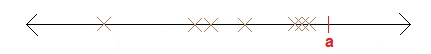
\includegraphics[width=18 cm]{images/upperbound.jpg}\\
\phantom{ } \hfill (Here, the $\times$s represent elements of $S$)\\
What the above diagram shows is that the number $a$ lies on the right of \textit{every} element of the set. It might now feel natural to write the definition that we saw before:
\begin{center}
    \highlight{$a$ is an upper bound of $S$ if: $\forall x \in S(x \le a)$}
\end{center}
Similarly, what can we say if $a$ is \textbf{\textit{not}} an upper bound of $S$? Once again, we may draw a number line as follows:\\
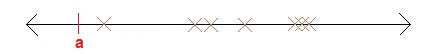
\includegraphics[width=18 cm]{images/lowerboundfalse.jpg}\\
In the above case, $a$ is certainly not the upper bound. However, is this the only way? The above diagram shows that $a$ is to the left of \textit{every} element of $S$. What if there's a situation like below:\\
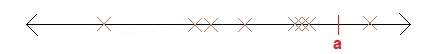
\includegraphics[width=18 cm]{images/lowerbound.jpg}\\
In this case as well, $a$ is \textit{\textbf{not}} an upper bound. Therefore, it not necessary that \textit{every} element of $S$ be greater than $a$, just \textit{one} would suffice. Now, we may write that:
\begin{center}
    \highlight{$a$ is not an upper bound of $S$ if: $\exists x \in S(a < x)$}
\end{center}
Of course, as we had already seen \hyperref[sec:negquant]{negating quantifiers} before, this was quite straightforward. The purpose of this activity had mainly been to illustrate the use of number lines and intuition.

\hrulefill
\exercise{Do the same for lower bounds.}

\hrulefill

\subsection{Proper way of writing a definition}\label{ssec:properdef}
\nopagebreak
\begin{enumerate}[label=(\arabic*)]
    \item Let $a\in \mathbb{R}, S\subset \mathbb{R}.$\\
    We say $a$ is a lower bound of $S$ \textbf{in $\mathbb{R}$} if:\\
    $\forall x \in S(a \le x).$
    %
    \item Let $S\subset \mathbb{R}$.\\
    We say that $S$ has a lower bound \textbf{in $\mathbb{R}$} if:\\
    $\exists a \in \mathbb{R}\big(\forall x \in S(a \le x)\big)$
\end{enumerate}

Just like how we'd negated a complicated statement, the procedure of writing a definition is quite similar.\\
Begin with the last line as you know what the property is supposed to be. 
\begin{center}
    \highlight{$\forall x \in S(a \le x).$}
\end{center}
The above statement involves three \textit{characters}: $x$, $S$ and $a$. It is clear what $x$ is as it's mentioned in the statement itself. The other two characters will have to be introduced. It is now immediately clear what we must write:
\begin{center}
    \highlight{%
    Let $a\in \mathbb{R}, S\subset \mathbb{R}.$\\
    $\forall x \in S(a \le x).$}
\end{center}
Now, all we are left with is just to tell the reader what is it that we are defining.
\begin{center}
    \highlight{%
    Let $a\in \mathbb{R}, S\subset \mathbb{R}.$\\
    We say $a$ is a lower bound of $S$ if:\\
    $\forall x \in S(a \le x).$}
\end{center}
Note that this line came second as the line uses the characters $a$ and $S$.\\
If you look at the two definitions above, you may notice that in the second definition, ``$a\in \mathbb{R}$" was not part of the introduction. This is correct because the third line tells us what $a$ is. (This is similar to how we never introduce $x$ before.)\\~\\
If you see the final statement of definition (2), the inner statement is just taken from the previous definition. This shows how one builds up definitions and that an intermediate step could have just been to write:
\begin{center}
    \highlight{$\exists a \in \mathbb{R}(a $ is a lower bound of $S)$}
\end{center}
Which is then followed by the definition of $a$ being a lower bound of $S$.
%
\section{Proofs versus Counterexamples}\label{sec:pvsce}
Consider the statement:
\begin{center}
    \simpleexample{Every non-empty subset of $\mathbb{R}$ has a lower bound in $\mathbb{R}$.\\
    That is: $\forall S \subset \mathbb{R}, S \neq \emptyset\Big(\exists a \in \mathbb{R}\big(\forall x \in S(a\le x)\big)\Big)$}
\end{center}
Is the above statement true? If yes, how would we show that? If no, then how would we show that?\\
The statement starts with the \hyperref[ssec:univquant]{"for all" quantifier}. Therefore, what it claims afterwards must hold for \textit{all} non-empty subsets $S$ for it to be true. This means that to show that it is false, all one would have to do is to find a single case where it does not hold, that is, a counterexample.\\
This reasoning is also consistent with the way we negated quantifiers before. Let us write the negation of the above statement.
\begin{center}
    \simpleexample{$\exists S \subset \mathbb{R}, S \neq \emptyset\Big(\forall a \in \mathbb{R}\big(\exists x \in S(x < a )\big)\Big)$\\
    That is: There is a non-empty subset of $\mathbb{R}$ that does \textit{not} have a lower bound in $\mathbb{R}$.}
\end{center}
Note an important thing: even in the negation, we're still saying \simpleexample{$S\neq\emptyset$}. This is because I made my original statement about non-empty subsets of $\mathbb{R}$; therefore, if you say that the inner-statement doesn't hold for the empty subset, you've not proven me wrong.\\
Another example of this would be:\\
\simpleexample{%
My claim: Chirag is the tallest student in this classroom.\\
To prove me wrong, you'd have to pick a \textit{\textbf{student}} in the room who is taller than Chirag. You would \textbf{\textit{not}} have proven me wrong if you pick some professor%
\footnote{ignoring the philosophical take that ``we're  all students in some way".}%
in the classroom and they happen to be taller than Chirag.
}\\
Now, going back to the original statement, let's try to prove it wrong. We have shown that all it would take to disprove the statement is to find a single counterexample. So, let us think of a non-empty subset that would not have a lower bound.\\~\\
In terms of the number line, what would this mean?\\
It would mean that no matter what real number $a$ that you choose, there would be an element of the set $S$ which is to the left of $a$. The picture would look something like:\\
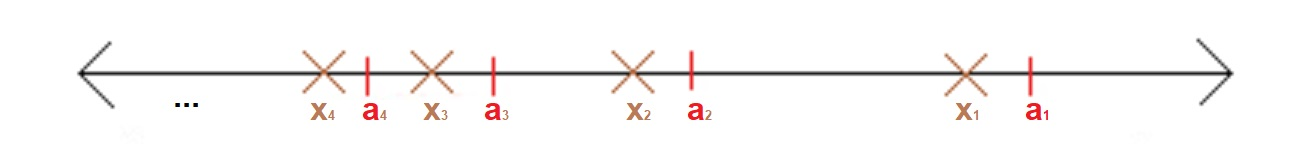
\includegraphics[width=18 cm]{images/nolowerbound.jpg}\\
Note that more than one element of $S$ can lie to the left of the $a$ you choose, the important thing is that \textit{at least} one does.\\
One simple counterexample can be $\mathbb{R}$ itself.

\hrulefill
\exercise{Given the above picture, come up with 5 counterexamples.}
\exercise{Prove that all the sets that you mentioned above do not have a lower bound in $\mathbb{R}$.}
\exercise{Is the statement true if we replace $\mathbb{R}$ with: (i) $\mathbb{N}$ (ii) $\mathbb{Z}$?}

\hrulefill

\highlight{\textbf{Claim: }
\begin{tabular}[t]{l}
     Let $S \subset \mathbb{R}, \cancel{S \neq \emptyset}$\\
     Suppose $S$ has a maximum.\\
     Then, $S$ is bounded above and $\operatorname{max}(S) = \operatorname{lub}(S)$.
\end{tabular}
}\\
In the above claim, I have struck out ``$S \neq \emptyset$", this is because that is redundant as $S$ having a maximum would imply that it's non-empty.\footnote{once again, recall that maximum demands the existence of a maximal element within the set itself.}\\
This is actually how one makes a theorem ``stronger". There are two ways of doing so:\\
(i) decrease the assumptions.\\
(ii) increase the conclusions.
%
\section{Well Ordering Principle}\label{sec:wop}
\highlight{\textbf{Axiom: }Every non-empty subset of $\mathbb{N}$ has a minimum.\\
That is: $\forall S \subset N, S \neq \emptyset\Big(\exists m \in S\big(\forall n \in S(m \le n)\big)\Big)$}\\
The above is known as well-ordering principle and is taken as an axiom.\\
It is easy to show that every subset of $\mathbb{N}$ would have a lower bound in $\mathbb{R}$. (1 would be a lower bound for every subset.) Well Ordering Principle is a stronger claim. If you feel it's obvious that a set having a lower bound should have a minimum, note that the same argument does not work for $\mathbb{Q}$.
%
\section{Intervals Notation}\label{sec:intervals}
Let $a, b \in \mathbb{R}$ for the following list:
\begin{enumerate}
    \item $(-\infty, \infty) = \mathbb{R}$
    \item $(-\infty, a) = \{x \in \mathbb{R}|x < a\}$
    \item $(-\infty, a] = \{x \in \mathbb{R}|x \le a\}$
    \item $(a, \infty) = \{x \in \mathbb{R}|a < x\}$
    \item $[a, \infty) = \{x \in \mathbb{R}|a \le x\}$
    \item $(a, b)$ 
    \begin{tabular}[t]{l}
        $=\{x \in \mathbb{R}|a < x$ and $x < b\}$  \\
        $=\{x \in \mathbb{R}|a < x\}$ and $\{x \in \mathbb{R}|x < b\}$ \\
        $=\{x \in \mathbb{R}|a < x\} \cap \{x \in \mathbb{R}|x < b\}$ \\
        $= (-\infty, b) \cap (a, \infty)$
    \end{tabular}
    \item $(a, b]= (-\infty, b] \cap (a, \infty)$
    \item $[a, b)= (-\infty, b) \cap [a, \infty)$
    \item $[a, b]= (-\infty, b] \cap [a, \infty)$
\end{enumerate}
Note that $\infty$ is just a symbol that has been used in some sort of notation, nothing more.
%
\chapter*{Assignment 2}\label{assign:2}
\addcontentsline{toc}{chapter}{Assignment 2}
\assign{21-01-2019}
\begin{enumerate}[label = (\arabic*)]
    \item Let $X$ be a set, $A, B \subset X, x\in X.$ Define (i) $A \cap B$ (ii) $A\cup B$ (iii) $A\subset B$ (iv) $A = B$
    %
    \item Write $A$ as a subset of $B$, where:
    \begin{enumerate}
        \item $A = \emptyset$;
        \begin{enumerate*}[label=(\roman*)]
            \item $B=\mathbb{R}$
            \item $B=\mathbb{Q}$
            \item $B=\mathbb{Z}$
            \item $B=\mathbb{N}$
        \end{enumerate*}
        \item $B=\mathbb{R}$;
        \begin{enumerate*}[label=(\roman*)]
            \item $A=(0, 1]$
            \item $A=\mathbb{Z}$
            \item $A=\mathbb{Q}$
        \end{enumerate*}
        \item $B=\mathbb{R}^2$; A is
        \begin{enumerate*}[label=(\roman*)]
            \item the $X-$axis
            \item the unit circle\\
            \item the set of solutions of the equation $x+2y=0$
        \end{enumerate*}
    \end{enumerate}
    %
    \item Describe the following sets:
    \begin{enumerate}
        \item 
        \begin{enumerate*}[label=(\roman*)]
            \item $\{x \in \mathbb{R}:x(x-1)(x-2)>0\}$
            \item $\{x \in \mathbb{R}:\cos(2\pi x) = 0\}$
            \item $\{x \in \mathbb{R}:x^2=1\}$
        \end{enumerate*}
        \item
        \begin{enumerate*}[label=(\roman*)]
            \item $\left\{(x, y)\in\mathbb{R}^2:\dfrac{x}{y}+\dfrac{y}{x} \ge 2\right\}$
            \item $\{(x^2, x):x\in\mathbb{R}\}$
        \end{enumerate*}
        \item $A \times B$, where
        \begin{enumerate*}[label=(\roman*)]
            \item $A = [0, \infty)$ and $B = [2, 3]$.
            \item $A = [3, 4]$ and $B = \mathbb{N}$.
        \end{enumerate*}
    \end{enumerate}
    %
    \item What is the st $A+2$, where
    \begin{enumerate*}[label=(\roman*)]
        \item $A = \mathbb{Z}$
        \item $A = \{1, 2, 3, 4\}$
        \item $A = [1, 2)$
        \item $A = (\infty, 0)$
    \end{enumerate*}\\
    What is the set $2A$ where $A$ is as above?\\
    What is the set $\frac{\pi}{4}(2\mathbb{Z} + 1)$? Is it related to any of the sets in the previous question?
    %
    \item What is the set $c + \mathbb{Q}$? When does it contain a rational number?\\
    What can you say in the other cases? Answer similar questions about $c\mathbb{Q}$.
    %
    \item Let $A$ and $B$ be non-empty subsets of $\mathbb{R}$, and $c \in \mathbb{R}$\\
    Describe the sets $-A, cA, c+A, A\cap B, A\cup B$ and $A+B$.\\
    How is their lub/glb (if they exist), related to the lub/glb of A and B?
    %
    \item Identify some rational and irrational numbers in $\mathbb{Q} + [0, 1]$? What is this set?
    %
    \item Let $S \in \mathbb{R}$. Is $S$ has a maximum, then $S$ is bounded above and $\operatorname{max}(S) = \operatorname{lub}(S)$.
\end{enumerate}

\hrulefill

Note: In (1), the first two sub-parts would require a set description while the last two would be a condition.
%
\chapter{Lecture 7}
\prs{23-01-2019}
Let's consider two sets, $S$ and $T$.\\~\\
\begin{tabular}{l|l}
    $S = \{x\in\mathbb{Q}|x^2\le 2, 0 < x\}$ & $T = \{x\in\mathbb{Q}|2\le x^2, 0 < x\}$ \\
    Is $S\neq\emptyset?$ & Is $T\neq\emptyset?$\\
    Yes. $1\in S$  & Yes. $3\in T$
\end{tabular}\\
Let us see what $S\cap T$ is.\\
$S\cap T $
\begin{tabular}[t]{l r}
    $= \{x\in\mathbb{Q}|x^2 \le 2$ and $2\le x^2, 0 < x\}$ & \\
    $= \{x\in\mathbb{Q}|x^2 = 2, x > 0\}$ & (Using Law of Trichotomy)\\
    $= \emptyset$ & (As we have proven that $\not\exists x\in \mathbb{Q} (x^2 = 2)$)
\end{tabular}\\
So, we have shown that $S$ and $T$ have no common elements. Is there any relation that we state between the elements of $S$ and $T$?

\hrulefill
\exercise{\label{ex:7.1}Prove that: $\forall s \in S, \forall t \in T(s < t)$}

\hrulefill

The set $S$ is bounded above in $\mathbb{Q}$, i.e., $\exists M \in \mathbb{Q}\big(\forall s\in S(s \le M)\big)$\\
The set $T$ is bounded below in $\mathbb{Q}$, i.e., $\exists m \in \mathbb{Q}\big(\forall t\in T(m \le t)\big)$\\
Let $U_{S\mathbb{Q}}$ be the set of all upper bounds of $S$ in $\mathbb{Q}$. By the \hyperref[ex:7.1]{above exercise}, we have: $T \subset U_{S\mathbb{Q}}$.\\~\\
Question: Is $T = U_{S\mathbb{Q}}?$\\
Attempt to solve: Let $x \in U_{S\mathbb{Q}}$.\\
Can $x \le 0$ be true? No. (Why?)\\
$\therefore U_{S\mathbb{Q}} \subset \{x\in\mathbb{Q}|0 < x\}$\\
Now, if there is some $y$ such that $y \not \in T$ but $y \in U_{S\mathbb{Q}}$, then: $y^2 < 2, 0 < y, y \in \mathbb{Q}$\\
The above is then equivalent to: $y\in S$.\\~\\
Next question: Can an element in $S$ be an upper bound of $S$ in $\mathbb{Q}$?\\
That is: Is $\exists M \in S\big(\forall s \in S(s\le M)\big)$ true?\\
The above is equivalent to asking: Does $S$ have a maximum?\\
Answer: As it turns out, no. $S$ does not have a maximum.\\
That is: $\forall M \in S\big(\exists s \in S(M < s)\big)$ is true.\\
What this means is:\\
\highlight{For any $a \in S$, there is an element $s_a \in \mathbb{Q}$ such that $a < s_a$ and $s_a^2 < 2$.}

\hrulefill
\exercise{Prove the above statement. That is, try to come up with a number $s_a \in \mathbb{Q}$ which depends on $a$ in such that a way that it is strictly greater $a$ than while having its square be strictly less than 2.\\
Hint: Write $s_a = a + a_0$ where $a_0$ is a positive rational such that $(a+a_0)^2 < 2$. Find an appropriate $a_0$. (This exercise is \textit{\textbf{not}} trivial. The purpose of this exercise is show how it's not easy to construct such a number algebraically.)}

\hrulefill

As we have ``shown" that $S$ does not have a maximum, it means that it is not possible for a $y$ to exist such that $y \not \in T$ but $y \in U_{S\mathbb{Q}}$.\\
This means that if $y \not \in T$, then $y \not \in U_{S\mathbb{Q}}$.\\
This means that if $y \in U_{S\mathbb{Q}}$, then $y \in T$.\\
Thus, we have shown that $U_{S\mathbb{Q}} \subset T$.\\
As we already knew that $T \subset U_{S\mathbb{Q}}$, we can now conclude: $\boxed{T = U_{S\mathbb{Q}}}$
\section{Least Upper Bound}\label{sec:lub}
\highlight{%
\textbf{Definition: }
Let $(X, <)$ be an ordered set. Then, $A\subset X$ is said to have a least upper bound (lub) $\alpha$ if $\alpha$ is an upper bound of $A$ in $X$ and $\alpha$ is smaller than all other upper bounds of $A$ in $X$.\\
}
$a\in X$ is the lub of $A \subset X$ if:
\begin{enumerate}[nosep]
    \item $\forall a \in A(a \le \alpha)$
    \item if $\exists \beta \in X\big(\forall a \in A(a \le \beta)\big)$, \hfill(Basically stating that $\beta$ is an upper bound)\\
    then $\alpha \le \beta$.
\end{enumerate}

\hrulefill
\exercise{In a similar manner, define greatest lower bound (glb) of $A\subset X$ where $(X, <)$ is an ordered set.}
\exercise{Find glb and lub (if they exist) of $A_i$ in $X_i$ in the following cases:
\begin{enumerate}[nosep]
    \item $A_1 = \{x \in \mathbb{Z}|-15<x<10\}$; $X_1 = \mathbb{Z}$
    \item $A_2 = \{x \in \mathbb{Q}|-15<x<10\}$; $X_2 = \mathbb{N}$
    \item $A_3 = \{x \in \mathbb{R}|-15<x<10\}$; $X_3 = \mathbb{R}$
\end{enumerate}
}

\hrulefill

Looking at the definition of lub, it tells us that $\alpha$ is an lub (of $A$ in $X$) if all other upper bounds (of $A$ in $X$) are greater than $\alpha$. However, while writing a proof, it is quite hard to work with that definition. Therefore, we can look at an equivalent condition which would be:
\begin{center}
    \highlight{Any number $(\in X)$ strictly less that $\alpha$ cannot be the upper bound (of $A$ in $X$).}
\end{center}
%
Let us look at half the solution of $\textbf{Ex 7.4.}$ 2.:\\
\claim{10 is the lub of $A_2$ in $\mathbb{Q}$.}{\\
(a) To show that 10 is \textit{an} upper bound.\\
Let $a \in A_2$.\\
By definition of $A_2, a < 10$.\\
$\therefore 10$ is an upper bound.\\
(b) To show that 10 is the \textit{least} upper bound.\\
Assume $\beta (\in \mathbb{Q}) < 10$ is an upper bound of $A_2$ in $\mathbb{Q}$.\\
As $-14\in A_2$, clearly $-15<-14\le\beta$ \hfill ---(I)\\
Consider: $\gamma = \dfrac{\beta+10}{2}$\\
As $\beta, 10 \in \mathbb{Q}$, this implies that $\gamma \in \mathbb{Q}$\hfill ---(II)\\
As $\beta < 10$, this means that $\beta < \dfrac{\beta+10}{2} < 10$ \hfill (Shown in \hyperref[assign:1]{Assignment 1})\\
$\implies \beta < \gamma < 10$ \\
$\implies -15 < \gamma < 10$ \hfill (Using (I))\\
The above, along with (II) gives us that: $\gamma \in A_2$\\
This means that $\beta$ cannot be an upper bound of $A_2$ as there exists an element ($\gamma$) in $A_2$ which is strictly greater than $\beta$.\\
This shows that any rational $\beta$ strictly less than 10 cannot be an upper bound of $A_2$.\\
$\boxed{\therefore 10\text{ is the lub of }A_2\text{ in }\mathbb{Q}.}$
}

This proof gives us a general idea of how one could go about to show that a number is the lub of a given set.\\
Let $(X, <)$ be an ordered set and let $A\subset X$.\\
$\operatorname{lub}(A) = \alpha$ if:
\begin{enumerate}[nosep]
    \item $\alpha$ is an upper bound.
    \item for any $\beta  (\in X)< \alpha$, $\exists a \in A(\alpha < a \le \beta)$
\end{enumerate}

\hrulefill

\exercise{Prove that lub of a set (if it exists) is unique.}

\hrulefill

Once you have shown that lub (and similarly glb) of a set (if it exists) is unique, it is appropriate to say ``\textit{the} lub". At the same time, one must say ``\textit{an} upper bound" when talking about an arbitrary upper bound. This is because one may use ``the" only when it is proven that the character is unique. Since there is no unique upper bound, one must not say ``\textit{the} upper bound".
%
\chapter{Lecture 8}
\pah{25-01-2019}
\section{Some subsets}\label{sec:subsets}
Let $X$ be a set and $A, B \subset X$.\\
Using these, we may construct some more subsets of $X$:
\begin{enumerate}
    \item \underline{Union}:
    \begin{enumerate}
        \item $A\cup B = \{x \in X|x\in A \text{ or } x \in B \}$
        \item $x \in A \cup B$ if $(x \in A$ or $x \in B)$
    \end{enumerate}
    \item \underline{Intersection}:
    \begin{enumerate}
        \item $A\cap B = \{x \in X|x\in A \text{ and } x \in B \}$
        \item $x \in A \cap B$ if $(x \in A$ and $x \in B)$
    \end{enumerate}
    
    In each case, both (a) and (b) mean the same but are useful in different scenarios. (b), for example, is useful when one wants to answer something like ``when is $x$ \textit{not} in the union/intersection?"
    %
    \item \underline{Complement}: Complement of $A$ is denoted by $A^c$
    \begin{enumerate}
        \item $A^c = \{x\in X|x\not\in A\}$
        \item Let $x \in X$\\
        $x\in A^c$ if $x \not \in A$
    \end{enumerate}
    Note that complement especially demands that $A$ should be part of a bigger set $X$. For union and intersection, one can construct them even if just $A$ and $B$ are given; however, given just $A$ without a larger set, $A^c$ is meaningless. This is also reflected by how (b) of complement starts with ``$x \in X$".
\end{enumerate}
\claim{$(A^c)^c=A$}{%
To show that: $A\subset(A^c)^c$ and $(A^c)^c \subset A$\\
First part:\\
Let $x \in A$. Now we must show: $x \in (A^c)^c$\\
If $x \in A$, then $x \not \in A^c$ \hfill (Follows from the contrapositive of the definition of $A^c$)\\
If $x \not\in A^c$, then $x \in (A^c)^c$ \hfill (Follows from the definition of $(A^c)^c$)\\
We have shown that $x \in A \implies x \in (A^c)^c$.\\
$\therefore A \subset (A^c)^c$\\
Second part:\\
Let $x \in (A^c)^c$. Now we must show $x \in A$\\
If $x \in (A^c)^c$, then $x \not \in A^c$ \hfill (Follows from the definition of $(A^c)^c$)\\
If $x \not \in A^c$, then $x \in A$ \hfill (Follows from the contrapositive of the definition of $A^c$)\\
We have shown that $x \in (A^c)^c \implies x \in A$.\\
$\therefore (A^c)^c \subset A$\\
This completes our proof.}

In the above proof, we have used something known as ``contrapositive".\\
If we have statement such as ``If p, then q", the contrapositive of that is ``If not q, then not p". The useful thing about contrapositive is that the contrapositive of a statement is logically equivalent to the original statement.\\
\example{%
Statement: $x \not \in A \implies x \in A^c$\\
Contrapositive: $x \not \in A^c \implies x \in A$
}\\~\\
Note: In the proof, we said that ``$x \in A \implies x \not\in A^c$"; this was the contrapositive of the definition as we take definitions to be ``if and only if" statements even though we do not write that.\\~\\
Going back to the above proof, what if we were not able to come up with the proof as given above? There is one way of proof often used which is called ``Proof by contradiction".  It starts by assuming that the opposite proposition is true, and then shows that such an assumption leads to a contradiction.%
\footnote{G. H. Hardy described proof by contradiction as ``one of a mathematician's finest weapons", saying ``It is a far finer gambit than any chess gambit: a chess player may offer the sacrifice of a pawn or even a piece, but a mathematician offers the game."}
If $P$ is the proposition to be proved:
\begin{enumerate}
    \itemsep0em
    \item $P$ is assumed to be false, that is $\sim P$ is true.
    \item It is shown that $\sim P$ implies  two mutually contradictory assertions, $Q$ and $\sim Q$.
    \item Since $Q$ and $\sim Q$ cannot both be true, the assumption that $P$ is false must be wrong, and $P$ must be true.
\end{enumerate}

Depicting that proof for the first part:\\
{\color{claimcolor}%
Let $x \in A$. Now we must show that $x \in (A^c)^c$.\\
Assume not. That is $x \in A$ and $x \not \in (A^c)^c$.\\
If $x \not \in (A^c)^c$, then $x \in A^c$.  \hfill (Follows from the contrapositive of the definition of $(A^c)^c$)\\
If $x \in A^c$, then $x \not \in A.$  \hfill (Follows from the definition of $A^c$)\\
This gives us that $x\in A$ and $x\not\in A$ which cannot be true.\\ Therefore, our assumption was wrong and $x \in (A^c)^c$ must be true.\\
This proves the first part that $x \in A \implies x \in (A^c)^c.$
}\\
Note that here we wanted to show that \textit{given} an $x$ belonging to $A$, $x \in (A^c)^c$. Which is why when we assumed that the proposition was false, we didn't negate $x \in A$ because that was part of the hypothesis.\\
In this case, the proof by contradiction was quite similar to the direct proof as almost identical arguments were made. In fact, looking at the proof by contradiction, one may even see how the direct proof would follow. Also note that in this case, the direct proof is neater and easier to follow.
%
\subsection{Relation between the subsets}\label{ssec:relsubset}
When given two real numbers, a natural question could be to ask whether they're equal. If not, which one is smaller?\\
A similar thing can be done with sets, where instead of ``smaller", we may ask whether one is a subset of the other. Except here, there's no law of trichotomy. That is, it is possible for two sets to be not equal as well as neither be a subset of the other.\\
Given \textit{any} two arbitrary subsets $A, B$ of a set $X$, it may not be possible to comment on their relation with each other but we \textit{can} comment on their relation with their union and intersection.
\begin{enumerate}
    \itemsep0em
    \item $A, B, A \cap B \subset (A \cup B)$
    \item $(A\cap B) \subset A, B$
\end{enumerate}
Combining the above two points, we may write:
\begin{center}
    \highlight{$(A\cap B)\subset A \subset (A\cup B)$}
\end{center}
No need to mention $B$ as it follows from symmetry. (How?)\\
The above statement actually implies two statements: $(A\cap B)\subset A$ \textit{and} $A \subset (A\cup B)$.

\hrulefill
\exercise{Prove the following:
\begin{enumerate}
    \itemsep0em
    \item $A \subset (A\cup B)$
    \item $(A\cap B) \subset A$
    \item $A\subset B$ and $B \subset C\implies A\subset C$; that is, $\subset$ is a transitive relation.
\end{enumerate}}

\hrulefill

After having defined such new sets, it might feel natural to ask some questions about them to look at their properties.\\
Let us do that by deciding the truth value of the following statements.\\~\\
S1. For any set $X$, given any $A, B \subset X$: $A\cap B = \emptyset$\\
Is the statement true or false?\\
As it's talking about \textit{all} $X$ and \textit{all} subsets of $X$, a way to show that the statement is false is to just come up with one $X$ and choose subsets $A$ and $B$ of $X$ such that $A\cap B\neq \emptyset$. (\hyperref[sec:pvsce]{Proofs versus Counterexamples.})\\
Come up with 3 such counterexamples yourself.\\
One counterexample: $X=A=B=\{1\}$. It can also be seen how this is the ``simplest" counterexample in terms of number of elements.\\
Therefore, S1 is $\boxed{\text{false.}}$\\~\\
S2. For any set $X$, given any $A, B \subset X$: $A\cap B = A$\\
Once again, to show that the above statement is false, one counterexample would suffice. Also, chances are one of the 3 counterexamples that you came up with previously would also be a counterexample for this. The counterexample that I mentioned, however, would not.  (Come up with one yourself if your previous counterexamples do not work.)\\
The fact that a counterexample does exist shows that S2 is also $\boxed{\text{false.}}$\\~\\
Even if a statement turns out to be false, sometimes it's fruitful to ponder as to how can the statement be modified such that it becomes true. In terms of the statement stated above, what we'd like to do is- come up with a condition that implies that $A\cap B = B$\\~\\
Question: When is $A\cap B = A$ true?\\
Attempt to solve: Following just from the definition of set equality, we can write that the above is true if $(A\cap B) \subset A$ and $A\subset(A\cap B)$. We can straight away observe that the condition ``$(A\cap B) \subset A$" is always true. (Stated above.) As it was an ``and" condition and one of the statements is known to be true, it depends only the second statement.\\
$(A\cap B) = A$ is true if and only if $A \subset (A\cap B)$.\\
This can be written as:\\
    \highlight{Let $X$ be a set and $A, B \subset X$.\\
    Then, the following are equivalent:
    \begin{enumerate}[nosep]
        \item $(A\cap B) = A$
        \item $A \subset (A\cap B)$
    \end{enumerate}
    }
Let us see if we can proceed any further, that is, solve the question: When is $A \subset (A\cap B)$ true?\\
Attempt to solve: Let $A \subset (A\cap B)$\\
$\implies \forall x \in A(x \in A\cap B)$\\
$\implies \forall x \in A(x \in A$ and $x \in B)$\\
\phantom{ }\hfill (Note that the inner ``$x \in A$" doesn't add any information as it's always true)\\
$\implies \forall x \in A(x \in B)$\\
What we have now written is the condition that $A\subset B$.%
\footnote{note that this could have directly been concluded using the fact $(A\cap B)\subset B$}\\
$\therefore A \subset (A\cap B) \implies A \subset B$\\
This is interpreted as $A \subset B$ being a necessary consequence of $A\subset(A\cap B)$ being true. What this means is that if $A \subset B$ is false, then $A \subset (A\cap B)$ is false as well. (Contrapositive)\\
The next natural question now is: Does $A \subset B$ ensure that $A\subset(A\cap B)$?\\
This is known as the ``converse". For the implication $P \implies Q$, the converse is $Q \implies P$. However, unlike contrapositive, the converse is not equivalent to the statement. This means that showing that a statement is true does not mean that its converse will also be true.\\
In this case, though, the converse also does happen to be true.\\
That is: $A\subset B\implies A \subset (A\cap B)$\\
\phantom{ }\hfill\textit{The proof is trivial and is left as an exercise to the reader.}\\~\\

Now that this has been ``proven", we can add it to the list of equivalencies:

\highlight{
\begin{enumerate}[nosep]
    \item $(A\cap B) = A$
    \item $A\subset (A\cap B)$
    \item $A\subset B$
\end{enumerate}
}
I am now adding two more claims:
\highlight{
\begin{enumerate}[nosep]
    \setcounter{enumi}{3}
    \item $B = (A\cup B)$
    \item $B^c\subset A^c$
\end{enumerate}
}
%
\section{Equivalence}\label{sec:equiv}
In the previous example, we had a set of statements which we said were equivalent. What it really means is that all those statements will have same the truth value. That is, if any one of them is true, all the others will be true as well. Speaking in terms of conditional statements, it means that between any two statements of the list, there is an ``if and only if" relation.\\
So, given $n$ statements, how would one prove that they're equivalent? One way to do so would be to simply take all combinations of 2 statements and prove that either implies the other one. This would consists of proving $2\cdot\dbinom{n}{2}$ ``elementary" statements.
\footnote{$\binom{n}{k} = ^{n}$C$_k=\frac{n!}{k!(n-k)!}$}
\\
Is there a better way? Well, yes, what we could do is proceed in a following manner:\\
1) Show that $1.\iff 2.$\\
2) Show that $2. \iff 3.$\\
.\\
.\\
.\\
n-1) Show that $n-1. \iff n.$\\
This reduces the work to proving $2\cdot(n-1)$ ``elementary" statements. It can be seen that this is better than the previous case as $\dbinom{n}{2}$ is a quadratic in $n$ while $(n-1)$ is linear. Just in the case of the above example with $5$ statements, the difference in the two methods is: $20 - 8 = 12$\\
Turns out that there's an even better way, you could proceed as follows:\\
1) Show that $1.\implies 2.$\\
2) Show that $2. \implies 3.$\\
.\\
.\\
.\\
n-1) Show that $n-1. \implies n.$\\
n) Show that $n. \implies 1.$\\
This now reduces the task to $n$ ``elementary" statements. (Note how they're not $\iff$ anymore)\\
As the order of the statements does not matter, it is convenient to arrange them in an order such that it becomes the easiest to conclude one statement from the other.\\
%
\chapter*{Assignment 3}\label{assign:3}
\addcontentsline{toc}{chapter}{Assignment 3}
\assign{28-01-2019}
\begin{enumerate}[label = (\arabic*)]
    \item Identify the set $A\subset \mathbb{N}$ given that: if $x \in A$, then $x+1\in A$. Justify your answer.
    %
    \item The \textit{absolute value} or \textit{mod} function is defined as follows: $\forall x \in \mathbb{R}$, define
    \[ |x| = \left\{
        \begin{array}{l l}
            x & \text{when } x \ge 0 \\
            -x & \text{when } x < 0 
        \end{array}
    \right. \]
    Identify the following sets:\\
    \begin{enumerate*}[label=(\roman*)]
        \item $\{x\in\mathbb{R}: |x| = 3\}$
        \item $\{x\in\mathbb{R}: |x| \le 3\}$
        \item $\{x\in\mathbb{R}: |x+5| \le 3\}$
    \end{enumerate*}
    %
    \item Find $\lub(A)$ and $\glb(A)$ in $B$ in the following examples, if they exist. If not, explain why they do not exist.
    \begin{enumerate}[nosep]
        \item $A=\mathbb{N}, B=\mathbb{N}$
        \item $A = \{x\in\mathbb{Z} : -1 \le |x+5| < 8\}, B = \mathbb{Z}$. Does your answer change if $B=\mathbb{R}$?
        \item $A = \{x\in\mathbb{Q} : -1 \le |x+5| < 8\}, B = \mathbb{Q}$. Does your answer change if $B=\mathbb{R}$?
        \item $A = \{x\in\mathbb{Q} : x\neq0, 1/x \in \mathbb{N}\}, B = \mathbb{Q}$. Does your answer change if $B=\mathbb{R}$?
    \end{enumerate}
    %
    \item Let $A\subset\mathbb{R}$ and $\alpha \in \mathbb{R}$ such that $\alpha$ in an upper bound of $S$ in $\mathbb{R}$. Show that the following statements are equivalent.
    \begin{enumerate}[nosep]
        \item $\alpha$ is the least upper bound of $A$ in $\mathbb{R}$.
        \item For every $\epsilon > 0 \in \mathbb{R}$, there exist $a \in A$ such that $\alpha - \epsilon < a \le \alpha$
        \item For every $t\in\mathbb{R}$ with $t < \alpha$, there exists $a\in A$ such that $t < a \le \alpha$.
    \end{enumerate}
    %
    \item Let $c \in \mathbb{R}; A, B \subset \mathbb{R}$ be bounded and non-empty. State whether the following are true or false. If true, prove it. If false, give a counter-example, and state and prove the corrected version.
    \begin{enumerate}[nosep]
        \item If $A\subset B$ then $\lub(A) = \lub(B)$.
        \item $\lub(A\cup B) = \min\{\lub(A), \lub(B)\}$
        \item $\lub(A\cap B) \rule{1cm}{0.15mm}\{\lub(A), \lub(B)\}$
        \item $\lub(cA) = c \lub(A)$
        \item $\lub(A+B) = \lub(A) + \lub(B)$
    \end{enumerate}
    %
    \item Let $X$ be a set, $A, B \subset X$. Show that the following are equivalent:\\
    \begin{enumerate*}[label=(\roman*)]
        \item $A\subset B$
        \item $A = A\cap B$
        \item $A \subset (A\cap B)$\\
        \item $B^c \subset A^c$
        \item $B = A\cup B$
        \item $(A\cup B)\subset B$
    \end{enumerate*}
    %
    \item Let $a, b, c, d \in \mathbb{N}$. State the following mathematically and write their negations:
    \begin{enumerate}[nosep]
        \item $c$ divides $a$. (Easier to think of: $a$ is a multiple of $c$).
        \item $c$ is a common divisor of $a$ and $b$,
        \item $d$ is a greatest common divisor of $a$ and $b$.
    \end{enumerate}
\end{enumerate}
%
\chapter{Lecture 9}\label{lec:9}
\prs{30-01-2019}
\section{lub Axiom}\label{sec:lubaxiom}
An ordered set $S$ is said to satisfy the lub axiom if for every non-empty subset $A \subset S$ which is bounded above in $S$, $\lub(A)$ in $S$ exists.\\~\\
\textbf{Theorem:} There exists an ordered field $\mathbb{R}$ which satisfies the $\lub$ axiom.

\hrulefill

It can be shown that $\mathbb{R}$ is unique up to ordered field isomorphism. That is, any other set that satisfies all the axioms A1-A10 as well as $\lub$ axiom is isomorphic to $\mathbb{R}$.

\hrulefill

We could earlier show that $\mathbb{N}$ is unbounded in $\mathbb{N}$ and $\mathbb{Q}$. (Refer: \hyperref[ex:unboundedN]{This} exercise.)\\
Now, we can show that $\mathbb{N}$ is not bounded above in $\mathbb{R}$. As we wish to show that existence of a certain element (that is, an upper bound) is \textit{not} possible, it may feel natural to prove it using contradiction.\\~\\
\textbf{Proposition}: $\mathbb{N} \subset \mathbb{R}$ is not bounded above in $\mathbb{R}$.\\
\textbf{Proof}: Assume the negation of the proposition. That is, let us assume that $\mathbb{N}$ \textit{is} bounded above in $\mathbb{R}$.\\
Then, by $\lub$ axiom, $\mathbb{N}$ has an $\lub$ in $\mathbb{R}$.\\
$\exists \alpha \in \mathbb{R}\bigg(\big(\forall n \in \mathbb{N}(n\le \alpha)\big)$ and $ \big(\forall 0< \epsilon (\in \mathbb{R}), \exists m \in \mathbb{N}(\alpha - \epsilon < m \le \alpha) \big)\bigg)$\\
Letting $\epsilon=1$ gives:
\begin{tabular}[t]{r l}
    $\exists m\in\mathbb{N}:$ & $\alpha - 1 < m \le \alpha$\\ 
    $\implies$ & $\alpha < m+1\le \alpha + 1$
\end{tabular}\\
But, if $m\in\mathbb{N}$, then $(m+1) \in \mathbb{N}$.\\
As $\alpha < m+1 (\in \mathbb{N})$, $\alpha$ is not an upper bound.\\
This is a contradiction and therefore, our original assumption was false which means that our proposition must be true. \hfill $\qed$\\~\\

In the above proof, we used $\epsilon = 1$, we could do this as the statement above said something true \textit{for all} $0 < \epsilon$, this gives us the liberty to choose any $\epsilon$ of our choosing. The reason why we thought $\epsilon=1$ might be helpful here was because we know that if $n$ is a natural number, then $n+1$ must also be a natural number.
%
\section{Archimedean Property}\label{sec:APoR}
$\mathbb{R}$ has the Archimedean property which states that:
\begin{enumerate}[nosep]
    \item $\forall x, y \in\mathbb{R}, 0 < x \big(\exists n \in \mathbb{N}(y < nx)\big)$
    \item $\mathbb{N}$ is not bounded above in $\mathbb{R}$.
\end{enumerate}

The two statements stated above are in fact, equivalent. 

\hrulefill

\exercise{Prove that the two statements are equivalent.}
\exercise{Prove or disprove that $\mathbb{Z}$ is bounded in: 
    \begin{enumerate*}[label=(\roman*)]
        \item $\mathbb{Z}$
        \item $\mathbb{Q}$
        \item $\mathbb{R}$
    \end{enumerate*}\\
    If your answer in any case is that is not bounded, then answer whether it is not bounded above as well as not bounded below.}
\exercise{Try to show that $\mathbb{Z}$ is not bounded below in $\mathbb{R}$ using the fact that $\mathbb{N}$ is not bounded above in $\mathbb{R}$.}
 
\hrulefill

Going back to a question of \hyperref[assign:3]{Assignment 3}, we had to find the $\lub$ and $\glb$ of the set:\\A = $\{x\in\mathbb{Q} : x\neq0, 1/x \in \mathbb{N}\}$\\
Looking at the set, it can be seen that it same as: $\left\{\left.\dfrac{1}{n}\right|n\in\mathbb{N}\right\}$\\
This makes it clear that $\lub(A)=1$ as $1$ is the maximum of the set.\\
It is clear that $A$ has no minimum. It can be seen that every element of $A$ is positive. Therefore, it is  clear that $0$ is a lower bound of the set. So, we may guess that $0$ is the $\glb$ of the set. For this we must show that:\\
$$\forall 0 < \epsilon (\in \mathbb{R}), \exists m\in \mathbb{N}\left(0 \le \dfrac{1}{m} \le 0 + \epsilon\right)$$

\hrulefill

\exercise{Show that $\glb(A)=0.$}

\hrulefill
\section{Abundance of Rational numbers}\label{sec:abundanceofq}
We would now like to prove that between any two real numbers, there always exists a rational number. That is:
$$\forall x, y \in\mathbb{R}, x < y\big(\exists q \in\mathbb{Q}(x < q < y)\big)$$
Since $q \in \mathbb{Q}$, it can be written as $\frac{m}{n}$ where $m, n \in \mathbb{Z}, 0 < n$. (We're not saying that $m$ and $n$ share no common factors, so $m$ and $n$ aren't fixed.)\\
$$x < \dfrac{m}{n} < y \iff nx < m < ny$$
So, the above question is now equivalent to showing that there exist two integers $m$ and $n$ satisfying $nx < m < ny$. This leads to asking: When can we ensure that there exists an integer between two real numbers?\\
Looking at some examples would lead us to believe that whenever difference of two real numbers is (strictly) greater than 1, then an integer will surely lie in between. (Strictly is required as there's no integer in $(1, 2)$)\\
Even though we haven't yet proven our above claim, let us first see if we \textit{can} in fact ensure that the difference is strictly greater than 1. That is: $1 < ny - nx$
$$1 < ny - nx \iff 1 < n(y-x)$$
As $1, (y-x) \in \mathbb{R}$ and $0 < y-x$, Archimedean property of real numbers says that there does exist a natural number $n$ satisfying that. (Note that we have no control over $x$ and $y$ but $m$ and $n$ are up to us for choosing.)\\~\\
All we have to now show is to prove our hypothesis, \textit{id est}- whenever difference of two real numbers is (strictly) greater than 1, then an integer will surely lie in between.

\hrulefill

\exercise{Try proving the above hypothesis.}

\hrulefill
%
\chapter{Lecture 10}
\pah{01-02-2019}
\section{Writing some proofs}\label{sec:writingproofs}
This lecture comprised of solving some problems which were given in \hyperref[assign:2]{Assignment 2}.\\

\hrulefill
\ \\~\\
Question. Write $A = \emptyset$ as a subset of $B = \mathbb{R}$.\\
Solution.\\
    $A = \{x\in\mathbb{R}|x^2 < 0\}$\\
    ``$x\in\mathbb{R}$" makes it clear that $A \subset \mathbb{R}$. Now, we must show that $A$ is empty.
    \begin{proof}
    Assume not. Then, $A \neq \emptyset$.\\
    Let $x \in A$.\\
    By definition, 
    \begin{tabular}[t]{l r r}
        $x^2 < 0$ & & (1)  \\
        $x \in \mathbb{R}$ & & \\
        $\therefore 0 \le x^2$ & [$\forall a \in \mathbb{R}(0 \le a^2)$] &(2)
    \end{tabular}\\
    By (1) and (2), we have:\\
    $x^2 < 0$ and $0 \le x^2$\\
    But $x \in \mathbb{R}$ implies that $x^2 \in \mathbb{R}$.\\
    Hence $x^2 < 0$ \textit{and} $0 \le x^2$ contradicts \hyperref[sec:LoT]{Law of Trichotomy of real numbers.}\\
    Thus, the assumption $A \neq \emptyset$ is incorrect and hence, $A = \emptyset$.
    \end{proof}

\dotfill
    
    Notes:
    \begin{enumerate}
        \item The above proof presented is a proof by contradiction.
        \item It was important to explicitly state that we are assuming ``$A \neq \emptyset$" as it makes the next line ``Let $x \in A$" valid. Moreover, it gives the clarity that all the reasoning that had followed was because we said ``$A \neq \emptyset$".
        \item When writing the reason for (2), we used another variable $(a)$. This was to show that the property we're using is \textit{for any} real number and therefore, it must be valid for $x$ too as it is a real number.
        \item We cannot directly conclude that ``$x^2 < 0$ and $0 \le x^2$" is a contradiction of Law of Trichotomy as it is a law about \textit{real numbers}. Therefore, first we must show that $x^2$ \textit{is} a real number. (Of course, later on, these things are always at the back of our mind and we need not write it.)
    \end{enumerate}

\hrulefill

\exercise{Show that $\{x \in \mathbb{R}|x^2 + 1 = 0\} = \emptyset$}

\hrulefill
\newpage
Question. Let $X$ be any set. Show that: $\emptyset \subset X$.\\
Solution.\\
To show that it is true, it is enough to show that its negation is false.\\
That is, prove that: $\emptyset \not\subset X$ is false.
\begin{proof}
Assume not. Then, $\emptyset \not\subset X$ is true.\\
Recall the condition for $A\subset B$: $x \in A \implies x \in B$.\\
The negation of that would be: $\exists x \in A$ such that $x \not\in B.$\\
Using that here, tells us that: $\exists x \in \emptyset$ such that $x \not\in X$.\\
But $\emptyset$ is empty. Hence, ``$\exists x \in \emptyset$" cannot be true which means the above statement cannot be true. Therefore, it is false.\\
As we concluded a false statement from our assumption, our assumption must be false as nothing false can follow from something true.\\
$\implies \emptyset \not\subset X$ is false $\implies \emptyset \subset X$.
\end{proof}

\dotfill

Notes:
\begin{enumerate}
    \item The above is proof is also a proof by contradiction.
    \item While working with empty sets, proofs usually take a route of contradiction as it is usually not possible to have a direct proof.
    \item Due to the nature of the empty set, a lot of statements about the empty sets are \textit{vacuously true.} Similarly, statements of the form ``If p, then q" are also vacuously true if p itself is false.
    Examples:
    \begin{enumerate}[nosep]
        \item ``All my children are cats" is a vacuous truth when spoken by someone without children.
        \item ``If $\sin(x)=x$, then $\pi = 3.$" is also a vacuous truth. \footnote{Despite what some \st{engineers} people might try to convince you, it is only \textit{vacuously} true.}
        \item ``All odd numbers divisible by 2 are prime."
        \item ``If the square of a real number is negative, then it is -1."
        \item ``If pigs fly, then they don't fly." \footnote{This was written at a time when pigs didn't fly. (Note that this does \textit{not} imply that pigs do fly at the time you're reading this.)}
    \end{enumerate}
\end{enumerate}

\hrulefill

\exercise{Recall the $\epsilon-\delta$ of limit and show that every function $f:\mathbb{N}\to \mathbb{R}$ is continuous.}
\exercise{The above exercise would then tell you that is possible for a function $f: \mathbb{N} \to \mathbb{R}$ to have different limits. You must have previously proven that ``the" limit of a function ($g:\mathbb{R} \to \mathbb{R}$) (if it exists) is unique. Can you see where that proof breaks in the case of $f:\mathbb{N}\to\mathbb{N}$?}

\hrulefill

(Note: The above two exercises were not actually given in class but I, the author find them interesting.)
\newpage
Question. Describe the set $A = \left\{(x, y) \in \mathbb{R}^2\left|\dfrac{x}{y}+\dfrac{y}{x} \ge 2\right.\right\}$\\
Solution.\\
As $(x, y)\in \mathbb{R}^2$, Law of Trichotomy tells us that us that we have three options each for $x$ and $y$ which gives us $2^3=8$ cases.\\
Straight away, we can see that it if $x=0$ or $y=0$, then it cannot be a solution as $\dfrac{x}{y}+\dfrac{y}{x}$ would not be defined.\\
Therefore, we have that $x\neq 0$ and $y\neq0$. This leaves us with 2 possibilities each for $x$ and $y$ with a total of $2^2=4$ cases.\\
Based on this bifurcation, we can look at the following subsets of $\mathbb{R}^2$:
\begin{enumerate}[nosep]
    \item $\{(x, y) \in \mathbb{R}^2|0 < x, 0 < y\}$
    \item $\{(x, y) \in \mathbb{R}^2|x < 0, 0 < y\}$
    \item $\{(x, y) \in \mathbb{R}^2|x < 0, y < 0\}$
    \item $\{(x, y) \in \mathbb{R}^2|0 < x, y < 0\}$
\end{enumerate}
The above are the first, second, third, and fourth quadrants, respectively.\\~\\
%
%
Claim 1: If $(x, y) \in$ I quadrant, then $(x, y) \in A$.
\begin{proof}
Let $(x, y) \in$ I quadrant.\\
$(x, y) \in$ I quadrant $\implies 0 < x, 0 < y$.\\
$(x-y)^2 \ge 0$ \hfill [$x-y \in \mathbb{R}$ and $\forall a \in \mathbb{R}(a^2 \ge 0)$]\\
$\implies x^2 - 2xy + y^2 \ge 0$\\
$\implies x^2 + y^2 \ge 2xy$\\~\\
$\implies \dfrac{x^2+y^2}{xy} \ge 2$\hfill $\left[0 < x, 0 < y \implies 0 < xy \implies 0 < \dfrac{1}{xy}\right]$\\~\\
$\implies \dfrac{x}{y} + \dfrac{y}{x} \ge 2$\\~\\
$\therefore (x, y) \in A$
\end{proof}
%
%
Claim 2: If $(x, y) \in$ II quadrant, then $(x, y)\not\in A$.
\begin{proof}Let $(x, y) \in$ II quadrant.
$(x, y) \in$ II quadrant $\implies x < 0, 0 < y$.\\
$x < 0 \implies \dfrac{1}{x} < 0$ \hfill $\left[\forall a \in \mathbb{R}\left(a < 0 \implies \dfrac{1}{a} < 0\right)\right]$\\
$\dfrac{1}{x} < 0 \implies \dfrac{y}{x} < 0$ \hfill (1) $\left[\forall a, b \in \mathbb{R}\left(a < 0, 0 < b \implies ab < 0\right)\right]$\\~\\
Also, \\
$0 < y \implies 0 < \dfrac{1}{y}$ \hfill $\left[\forall a \in \mathbb{R}\left(0 < a \implies 0 < \dfrac{1}{a} \right)\right]$\\
$0 < \dfrac{1}{y} \implies \dfrac{x}{y} < 0$ \hfill $\left[\forall a, b \in \mathbb{R}\left(a < 0, 0 < b \implies ab < 0\right)\right]$\\~\\
$\implies \dfrac{x}{y} + \dfrac{y}{x} < \dfrac{y}{x}$ \hfill [Ordered Field Axiom (\refaxiom{8})]\\~\\
$\implies \dfrac{x}{y} + \dfrac{y}{x} < 0$ \hfill [Using (1) and transitivity of $`<'$]\\~\\
$\implies \dfrac{x}{y} + \dfrac{y}{x} < 2$ \hfill [Using transitivity and the fact that $0<1<1+1=2$]\\~\\
$\therefore (x, y) \not \in A$ \hfill $\Bigg[$Using Law of Trichotomy on $\dfrac{x}{y} + \dfrac{y}{x}\Bigg]$
\end{proof}
%
%
Claim 3: If $(x, y) \in$ III quadrant, then $(x, y) \in A$.
\begin{proof}
As $\dfrac{x}{y} + \dfrac{y}{x} = \dfrac{-x}{-y} + \dfrac{-y}{-x}$, this implies $(x, y) \in A\iff(-x, -y) \in A$\\\phantom{ } \\
$(x, y) \in$ III quadrant $\implies x < 0, y < 0 \implies 0 < -x, 0 < -y \implies (-x, -y) \in$ I quadrant $\implies (-x, -y) \in A \implies (x, y) \in A$\\~\\
\end{proof}
%
%
Claim 4: If $(x, y) \in$ IV quadrant, then $(x, y)\not\in A$.
\begin{proof}
As $\dfrac{x}{y} + \dfrac{y}{x} = \dfrac{y}{x} + \dfrac{x}{y}$, this implies $(x, y) \in A\iff(y, x) \in A$\\ \phantom{ }\\
$(x, y) \in$ IV quadrant $\implies 0 < x, y < 0 \implies (y, x) \in$ II quadrant $\implies (y, x) \not\in A \implies (x, y) \not\in A$.
\end{proof}
Let $B = \{(x, y) \in \mathbb{R}^2|(x, y) \in $I quadrant or $(x, y) \in $III quadrant$\}$\\
Claim 5: $A = B$
\begin{proof}
For $A=B$: $A \subset B$ and $B \subset A$\\
Claims 1 and 3 show that $B \subset A$.\\
Claims 2 and 4 along with the fact that $x\neq0$ and $y\neq0$ show that $B^c\subset A^c$. (Here complement in taken with respect to the bigger set being $\mathbb{R}^2$.)\\
Therefore, $A \subset B$ \hfill [$A\subset B \equiv B^c\subset A^c$]\\
$\therefore A = B$
\end{proof}
The $B$ above is precisely the description desired.

\dotfill

Notes:
\begin{enumerate}
    \item A way to start would be to look at some examples, see which points belong to the set $A$ and which do not. This would lead to the discovery that points of the form $(x, 0)$ and $(0, y)$ would not be in the set $A$, not because they don't satisfy the inequality but because the terms are not defined.
    \item The proof was written in a sequential manner covering all the quadrants in order. This is the cleaned up version. While in reality, the quadrants first covered were quadrants 2 and 4 as it was clear how any point in those quadrants could possibly not be in $A$.
    \item The proof of claim 1 might seem very weird as it seems to come seemingly out of nowhere. It was actually derived in a ``backwards" manner. That is, we assumed that there's an $(x, y)$ in the first quadrant which is in $A$, this then gave us:\\~\\
    $\dfrac{x}{y} + \dfrac{y}{x} \ge 2$\\~\\
    The most natural thing now was to take the LCM and see if that gets us somewhere:\\~\\
    $\dfrac{x^2 + y^2}{xy} \ge 2$\\~\\
    $(x, y)$ being in the first quadrant ensured that $xy$ was positive, this then let us multiply both sides with $xy$, which, after a bit of manipulation gave us:\\
    $(x-y)^2 \ge 0$- which is true for all $(x, y) \in \mathbb{R}^2$. However, coming till this result involved a step which we could do because we assumed $(x, y)$ to be in I quadrant. Writing these steps in the reverse direction very clearly proved our claim.
    \item After proving it for the first quadrant, it was quite an easy step to conclude Claim 3 from that, noticing the symmetries. Even if not the symmetry, we can observe that the only place we used that $(x, y)$ was in the first quadrant was when we multiplied both sides with $xy$. We can still do that for a point in the third quadrant as the product $xy$ would still be positive.
\end{enumerate}

\hrulefill

\exercise{Using the above method, describe the set $A = \{x \in \mathbb{R}| x(x-1)(x-2) < 0\}.$ Be sure that if you describe it as a set $B$, you have shown that $A=B$ and not just $A \subset B.$}

\hrulefill

\section{Cartesion Product}\label{sec:cartproduct}
\textbf{Definition: }Given sets $A, B$, we define:\\
\phantom{Definition: D}$A \times B = \{(a, b)|a \in A$ and $b \in B\}$\\~\\
\example{Let $A = \{1, 2\}, B = \{a, b\}$.\\
Then, $A\times B = \{(1, a), (1, b), (2, a), (2, b)\}$\\
$B \times A = \{(a, 1), (a, 2), (b, 1), (b, 2)\}$}\\
\example{All points $(x, y)$ in the XY plane are elements of $\mathbb{R}^2 = \mathbb{R}\times\mathbb{R}$}\\
\example{$\mathbb{N}\times\mathbb{R}$ is the set of all pairs $(a, b)$ where $a$ is a natural number and $b$ is a real number.}

\hrulefill
%
\chapter*{Assignment 4}\label{assign:4}
\addcontentsline{toc}{chapter}{Assignment 4}
\assign{04-02-2019}
\begin{enumerate}[label=(\arabic*)]
    \item Let $X, Y$ b non-empty sets, $A\subset X, B \subset Y$. Show that $A\times B$ is a subset of $X \subset Y$.
    %
    \item Find $A\times B\subset \mathbb{R}^2$, where\\
    \begin{enumerate*}[label=(\roman*)]
        \item $A=(0,1),$ $B=\mathbb{R}$
        \item $A = \{0, 1\},$ $B = \mathbb{R}$
        \item $A = \mathbb{N},$ $B = \mathbb{R}$\\
    \end{enumerate*}
    How do your answers change when 
    \begin{enumerate*}[label=(\roman*)]
        \item $A$ and $B$ are interchanged.\\
        \item $B=\mathbb{R}$ is replaced by $B = \mathbb{Z}$?
        \item $B = \mathbb{R}$ is replace by $[0, \infty)$
    \end{enumerate*}
    %
    \item Prove or disprove: Let $Z\subset X\times Y$. Then there  are subsets $A$ and $B$ of $X$ and $Y$ respectively such that $Z = A \times B.$
    %
    \item What is the set $c + \mathbb{Q}$ where $c \in \mathbb{R}$? When does it contain a rational number?\\
    What can you say in other cases? Answer similar questions about $c\mathbb{Q}$.
    %
    \item Identify some rational and irrational numbers in $\mathbb{Q} + [0, 1]$? What is this set?
    %
    \item Find the $\lub$ and $\glb$ of the following sets in $\mathbb{R}$ if they exist. Give an argument supporting your answer.
    \begin{enumerate}[nosep]
        \item $\{1/2^q \in \mathbb{R}|q\in\mathbb{Z}\}$
        \item $\{x \in \mathbb{R}|x < 1/n$ for some $n \in \mathbb{N}\}$
        \item $\{x \in \mathbb{R}| x > 1/n$ $\forall n\in \mathbb{N}\}$
    \end{enumerate}
    %
    \item Let $S \subset \mathbb{R}$. If $\lub(S) = a$, then show that $\glb\big(\{-s\in\mathbb{R}|s\in S\}\big)=-a.$
    %
    \item Let $S \subset \mathbb{R}$ be a bounded subset of $\mathbb{R}$. Let $T = \{s^2\in\mathbb{R}|s\in S\}$. Does it follow that $\lub(T)=(\lub(S))^2?$ If yes, prove it. If false, give a counterexample, correct the statement and then prove the corrected statement.
\end{enumerate}
%
\chapter{Lecture 11}
\prs{07-02-2019}
\section{The Floor Function}\label{sec:floor}
By the end of \hyperref[lec:9]{Lecture 9}, we had to show that if $1 < ny - nx$, then there is an integer $m$ such that $nx < m < ny$. To do that, we shall try to define the floor function. \footnote{in case this name sounds new, you may have heard this under the name ``Greatest Integer Function"}\\%
What we would like to show is:
$$\forall x \in \mathbb{R}, \exists ! M \in \mathbb{Z} \text{ such that: } M \le x < M + 1$$
The above $M$ would then be equal to the floor of $x$.
($``\exists!"$ isn't really standard notation, it stands for ``there exists a \textit{unique}")\\
\begin{proof} Let $S = \{k \in \mathbb{Z}|k \le x\}$\\
$S\neq\emptyset$ as $\mathbb{Z}$ is not bounded below. \hfill (Why does that mean $S\neq\emptyset$?)\\
$S$ is bounded above in $\mathbb{R}$ as $x$ is an upper bound.\\
$\therefore$By the \hyperref[sec:lubaxiom]{lub axiom}, $S$ has an $\lub$ in $\mathbb{R}$.\\
Let $\lub(S)=\alpha$.\\
The above means that: $\forall\epsilon \in \mathbb{R}, 0 < \epsilon \big(\exists M \in S(\alpha - \epsilon < M)\big)$\\
Letting $\epsilon = 1$, we get that:
\begin{flalign*}
    \exists M \in S \text{ such that: } & \alpha - 1 < M &\\
                                \implies & \alpha < M + 1 &
\end{flalign*}
As $\alpha$ is an upper bound of $S$, $\alpha < M+1$ implies that $(M+1) \not \in S$.
\begin{flalign*}
    \text{We know: } &\forall k \in S (k \le \alpha) & [\because \alpha \text{ is an upper bound}] &\\
    \implies & \forall k \in S (k < M+1) & [\because \alpha < M+1] & \\
    \implies & \forall k \in S (k \le M) & [\because S \subset \mathbb{Z} \text { and } (M+1) \in \mathbb{Z}] &\\
    \implies & M \text{ is the maximum of } S.
\end{flalign*}
$M$ is the maximum of $S \implies M$ is the $\lub$.\\
Now that we have shown the existence, it is easy to show that such an $M$ is unique by considering $M'<M$ and $M'>M$.
\end{proof}
Now, we can define the following function:
$$\lfloor \text{ } \rfloor: \mathbb{R} \to \mathbb{Z}$$
$$\floor{x}:= \lub\big(\{k \in \mathbb{Z}| k \le x\}\big)$$

\newpage
\begin{enumerate}
    \item $\floor{x}$ is the greatest integer which is lesser than or equal to $x$.
    \item The ``ceil" function is defined in a similar manner. It gives the least integer which is greater than or equal to $x$. It is denoted by $\lceil x \rceil$.
    \item You may have seen floor$(x)$ being denoted by $[x]$ but $\floor{x}$ is more accepted. $[x]$ is sometimes used to denote the ``nearest integer function". Verify that $[x] = \floor{x + 0.5}.$ (Where the rule that numbers of the form $z + 0.5$ are rounded up to $z+1$ for $z \in \mathbb{Z}$.) 
\end{enumerate}
%
\chapter{Lecture 12}
\pah{08-02-2019}
In Lecture 10, we defined \hyperref[sec:cartproduct]{the cartesian product}. Such a product makes it useful for notation.\\
\example{Archimedean Property: $\forall x, y \in \mathbb{R}, x > 0 \big(\exists n \in \mathbb{N}(y < nx\big)$\\
It can be written as:\\
$\forall x, y \in (0, \infty) \times \mathbb{R}\big(\exists n \in \mathbb{N}(y < nx\big)$}\\~\\
\textbf{Definition: }Let $(x_1, y_1), (x_2, y_2) \in X \times Y$.\\
\phantom{Definition: I} Then, $(x_1, y_1) = (x_2, y_2)$ if $x_1 = x_2$ and $y_1 = y_2$.\\~\\
Similar to $\mathbb{R}^2$, one may also consider $\mathbb{R}^3$ or in general, $\mathbb{R}^n$.\\
One of the benefits of considering such sets is that it becomes easier to represent data. \\
For example, let us consider the equation of a line (in $\mathbb{R}^3$) in vector form.\\
$L = \{\textbf{a} + \lambda\textbf{m}|\lambda \in \mathbb{R}\}$ for some $\textbf{a}, \textbf{m} \in \mathbb{R}^3$.\\
Here $L$ is the set of position vectors of all those points on the line passing through $\textbf{a}$ parallel to $\textbf{m}$.\\~\\
Let $\textbf{a} = (x_1, y_1, z_1)$ and $\textbf{m} = (a, b, c)$, then each point $(x, y, z) \in L$ is of the form $(x_1 + \lambda a, y_1 + \lambda b, z_1 + \lambda c)$.\\
Equating each co-ordinate gives us:\\
\(\begin{array}{rccc}
    & x = x_1 + \lambda a & y = y_1 + \lambda b & z = z_1 + \lambda c \\
    \implies & x - x_1 = \lambda a & y - y_1 = \lambda b & z - z_1 = \lambda c \\
\end{array}\)\\
Assuming $abc\neq0$, we can find the value of $\lambda$ from each equation, equating those values gives us:
$$\dfrac{x-x_1}{a}=\dfrac{y-y_1}{b}=\dfrac{z-z_1}{c}$$
Thus, it can be seen how the same line can be written in two different forms. Expressing it in terms of vectors in $\mathbb{R}^3$ gives a much more concise way.\\
Also, by our way of defining equality, it can be seen that the order matters and that $(1, 2) \neq (2, 1)$.\\~\\
If we look at the equation: $x_1 + 2x_2 + 3x_3 = 6$, three of its infinitely many solutions are:
\begin{enumerate*}[label=(\roman*)]
    \item $(6, 0, 0)$
    \item $(0, 3, 0)$
    \item $(0, 0, 2)$
\end{enumerate*}\\
As can be seen, it is important to list them in the correct order. $(6, 0, 0)$ is a solution while $(0, 0, 6)$ is not.\\~\\
Another example can be given which would work well with those who are familiar with a tailor-%
\footnote{This example was given to Professor by a person who was in his 70s when he gave this example, who was in turn given this example by his professor.}%
when a tailor takes measurements, (s)he doesn't keep mentioning the part they are measuring but rather just note down the measurements in a certain order. This is because the tailor knows what is the pre-decided order. This is why you don't end up with disproportionate clothes.
\section{Indexing Set}\label{sec:indexset}
An index set is a set whose members label (or index) members of another set.\\
For example, if we want a set $S$ which is the set of all IPL players, we may use an index set $T=$ set of all IPL teams, then:
$$S = \bigcup_{t \in T}(\text{set of players of }t)$$
Similarly, let $B$ = set of branches in IITB
$$\text{Set of all first year students in IITB} = \bigcup_{b\in B}(\text{Set of first year students in }b)$$
Let us now try to write $\mathbb{R}$ as a union of two sets. This can be done in many ways:
\begin{align*}
    \mathbb{R} &= (-\infty, 0) \cup [0, \infty)\\
    &= \mathbb{Q} \cup (\mathbb{R}\setminus\mathbb{Q})\\
    &= \mathbb{R} \cup \mathbb{R}\\
    &= \mathbb{R} \cup \emptyset\\
    &= (-\infty, 1] \cup [0, \infty)\\
\end{align*}
It can be seen that it's not a necessity for the sets to be disjoint, non-empty or a proper subset. However, in most cases, we do work with proper subsets whenever taking union.\\
Let us write $\mathbb{R}$ as a union of three sets:
\begin{align*}
    \mathbb{R} &= (-\infty, 0) \cup \{0\} \cup (0, \infty)\\
    &= \{0\}\cup\{1\}\cup(\mathbb{R}\setminus\{0, 1\})\\
\end{align*}
Let us write $\mathbb{R}$ as a union of sets indexed by integers:
\begin{align*}
    \mathbb{R} &= \bigcup_{z\in\mathbb{Z}}[z, z+1)\\
    &= \bigcup_{z\in\mathbb{Z}}(z, z+1]\\
    &= \bigcup_{z\in\mathbb{Z}}[z, z+1]\\
\end{align*}
The difference in the last way is that here some elements may appear in more than one sets but it is still valid.\\
What is \textbf{not} valid is the following: $\mathbb{R} = \displaystyle\bigcup_{z\in\mathbb{Z}}(z, z+1)$\\
Before showing why this not valid, we must see what it means for an element to lie in the union of infinitely many sets.\\
\textbf{Definition: }Let $\Lambda$ be an indexing set.\\
\phantom{Definition: D}$x \in \displaystyle\bigcup_{\lambda\in\Lambda}A_\lambda\iff\exists\lambda\in\Lambda(x\in A_\lambda)$\\
Similarly, one can naturally define intersection for infinitely many sets:\\
\textbf{Definition: }Let $\Lambda$ be an indexing set.\\
\phantom{Definition: D}$x \in \displaystyle\bigcap_{\lambda\in\Lambda}A_\lambda\iff\forall\lambda\in\Lambda(x\in A_\lambda)$\\~\\
\claim{$\mathbb{R}\neq\displaystyle\bigcup_{z\in\mathbb{Z}}(z, z+1)$}{If can take an element of $\mathbb{R}$ and show that it is not in the union, then we would be done.\\
Let us take $0\in\mathbb{R}$.\\
To show: $0\not\in\displaystyle\bigcup_{z\in\mathbb{Z}}(z, z+1)$\\
Proof: Assume not.
\begin{align*}
    0\in\displaystyle\bigcup_{z\in\mathbb{Z}}(z, z+1) &\implies \exists z_0 \in \mathbb{Z}\big(0\in(z_0, z_0+1)\big)\\
    &\implies \exists z_0 \in \mathbb{Z}\big(z_0 < 0 < z_0 + 1\big)\\
    &\implies \exists z_0 \in \mathbb{Z}\big(0 < -z_0 < 1\big)\\
\end{align*}
If $z_0\in\mathbb{Z}$, then $-z_0\in\mathbb{Z}$. Therefore, the above tells us that there lies an integer in the interval $(0, 1)$ which is a contradiction. (Why?)\\
Hence, $0\not\in\displaystyle\bigcup_{z\in\mathbb{Z}}(z, z+1)$ \hfill \qed
}

\hrulefill

\exercise{Write $\mathbb{R}$ as a union of sets where the sets are indexed by $\mathbb{N}$. (Try making the sets pairwise disjoint)}
\exercise{Write $\mathbb{R}$ as a union of sets where the sets are indexed by $\mathbb{R}$. (Try making the sets pairwise disjoint)}
\exercise{Write $\mathbb{R}^2$ as a union of 
\begin{enumerate*}[label=(\roman*)]
    \item lines
    \item circles
\end{enumerate*}\\
In each case, try to make the sets pairwise disjoint and come up with a \textit{good} indexing set.}

\hrulefill
%
\chapter{Lecture 13}
\prs{11-02-2019}
\section{Density of rationals}\label{sec:ratdense}
\highlight{\textbf{Theorem:} Between any two (distinct) real numbers, there exists a rational numbers.}
$$\forall x, y \in \mathbb{R}, x < y \big(\exists q \in \mathbb{Q}(x < q < y)\big)$$
\begin{proof}
The given statement is equivalent to saying:\\
$\exists m \in \mathbb{Z}, n \in \mathbb{N}(nx < m < ny)$\\
By \hyperref[sec:APoR]{the Archimedean Property of real numbers}, we know that:\\
$\exists n \in \mathbb{N}\big(1 < n(y-x)\big)$\\
$\iff \exists n \in \mathbb{N}\big(1 < ny - nx\big)$\\~\\
Let $k = \floor{nx}$\\
$\therefore k \le nx < k+1$ \hfill [By definition of floor function]\\
$\implies k + 1 \le nx + 1$\\
$\implies (k+1) - nx \le 1$\\
$\implies (k+1) - nx < ny -nx$ \hfill [$\because 1 < ny-nx$]\\
$\implies k + 1 < ny$\\
We also know that $nx < k+1$, this gives us that:\\
$nx < k+1 < y$\\
Letting $m = k+1$ gives us exactly what we wanted, completing the proof.
\end{proof}

\hrulefill

Note: Had we chosen $k' = \floor{ny}$, we wouldn't have gotten the strict inequality as we desired. Instead, we would have gotten: $nx < k' \le ny$

\hrulefill

\exercise{If we had taken the other route and chosen $k' = \floor{ny}$, we would have ended up with the following result:\\
$\forall x, y \in \mathbb{R}, x < y \big(\exists q \in \mathbb{Q}(x < q \le y)\big)$\\
Using this, prove the theorem.}

\hrulefill
\newpage
\section{Existence of n$^\text{th}$ root}\label{sec:rootn}
\highlight{\textbf{Theorem:} Let $\alpha \in \mathbb{R}, \alpha > 0$\\
\phantom{Theorem: T}Then, for any $n\in\mathbb{N}: \exists x \in \mathbb{R}$ such that $x^n = \alpha$}\\
\textit{Construction of proof.}\\
Let $S = \{x \in \mathbb{R}|x^n \le \alpha\}$\\
We would now like to use the $\lub$ axiom. To use that, we must first show that $S \neq \emptyset$ and that  $S$ is bounded above.\\
It is easy to see that $S \neq \emptyset$ as $0 \in S$.\\
However, later on, we'll see that we require the $\lub$ of this set to be positive. Therefore, we would like to show the existence of a positive real number in this set.\\
By Archimedean Property, we have that:\\
$\exists k \in \mathbb{N}\left(\dfrac{1}{\alpha} < k\right)$\\~\\
$\iff\exists k \in \mathbb{N}\left(\dfrac{1}{k} < \alpha\right)$\\~\\
$\implies\exists k \in \mathbb{N}\left(\dfrac{1}{k^n} \le \dfrac{1}{k} < \alpha\right)$ \hfill [$\because 1 \le k]$\\~\\
$\implies \exists k \in \mathbb{N}\left(\dfrac{1}{k} \in S\right)$\\~\\
Now, we would like to show that $S$ is bounded above.\\
$0 < \alpha \iff 1 < \alpha + 1 \implies \alpha + 1 < (\alpha + 1)^n \implies \alpha < (\alpha + 1)^n$\\
$\implies \forall x \in S\big(x^n < (\alpha + 1)^n\big)$\\
$\implies \forall x \in S\big(x < \alpha + 1\big)$ \hfill (*)\\
$\therefore S$ is bounded above.\\~\\
Therefore, by the $\lub$ axiom: $\exists \beta \in \mathbb{R}$ such that $\lub(S) = \beta$.\\
Now, we would like to claim that $\beta^n = \alpha$\\
As it does not seem feasible to prove it directly, we may try proving it via contradiction. That is, show that $\beta^n \neq \alpha$ is not possible. This would give us two cases that we'd have to disprove:\\
(i) $\beta^n < \alpha$\\
(ii) $\alpha < \beta^n$\\~\\
Case (i): $\beta^n < \alpha$\\
As $\beta$ is the $\lub$, in order to reach a contradiction, there could be two possible things that we could contradict. Either the fact that $\beta$ is an upper bound itself or that $\beta$ is the \textit{least} upper bound. \\
Given our existing intuition of real numbers, it might feel that the path to the contradiction in this case would be to show the existence of a $\beta'$ such that $\beta^n<\beta'^n<\alpha$ which would give us that $\beta < \beta'$ (*) resulting in the contradiction that $\beta$ is an upper bound.\\~\\
Phrasing it in other manner, we would like to show the existence of a real number $h > 0$ such that $(\beta + h)^n < \alpha$. Phrasing it this way is nicer as it already ensures that the new number is strictly greater than $\beta$ and also makes it easier to work with it.\\~\\
\begin{flalign*}
(\beta+h)^n &= \beta^n + \dbinom{n}{1}\beta^{n-1}h + \dbinom{n}{2}\beta^{n-1}h^2 + \dots h^n&\\
\end{flalign*}
Our aim now would be to get an expression that is greater than $(\beta + h)^n$ which we can easily make lesser than $\alpha$ by choosing $h$ appropriately. Note that this must be done in a ``nice" manner.\\
As it is difficult to work with higher powers, we could try to convert the expression above to be linear in $h$. As we want the resulting expression to be greater, we would need \highlight{$h \le 1$}. We can do this as we have the luxury to choose $h$.\\
\begin{flalign*}
(\beta+h)^n &= \beta^n + \dbinom{n}{1}\beta^{n-1}h + \dbinom{n}{2}\beta^{n-1}h^2 + \dots h^n&\\
&\le \beta^n + \dbinom{n}{1}\beta^{n-1}h + \dbinom{n}{2}\beta^{n-1}h + \dots h&\\
&= \beta^n + h\underbrace{\left[\dbinom{n}{1}\beta^{n-1} + \dbinom{n}{2}\beta^{n-1} + \dots 1\right]}_{t_0} &\\
&=\beta^n + ht_0&\\
\end{flalign*}
We now wish to make $\beta + ht_0$ smaller than $\alpha$. Note that $t_0$ is a fixed quantity over which we have no control. We can, however choose $h$ accordingly.\\
It is clear that if we take $h$ to be any positive real number less than $\dfrac{\alpha-\beta^n}{t_0}$, we'll get the required inequality. As the numerator and denominator both are positive, it would be easy to show that such a number does exist.\\~\\
By Archimedean Property, $\exists M \in \mathbb{N}$ such that $t_0 < M\cdot(\alpha - \beta^n)$ \hfill [$\because \alpha - \beta^n > 0$]\\
Letting $h = \dfrac{1}{M}$ would then work. Recall that along the way, we did claim that $h \le 1$. Therefore, we must ideally say that $h = \min\left\{\dfrac{1}{M}, 1\right\}$. In this case, however, it won't matter as $M$ is a natural number.\\~\\
This we have now shown the existence of a positive real number $h$ such that $(\beta+h)^n < \alpha$.\\
$\therefore \beta + h \in S$.\\
This contradicts that $\beta$ is an upper bound. Therefore, $\beta^n < \alpha$ is not possible.

\dotfill

Note that the above way of writing was an informal way to see how one would work through it all. The ``proper" proof would work in a somewhat backwards manner. I shall now write the proof of the second case.

\dotfill

Case (ii): $\alpha < \beta^n$\\~\\
Let $t_0 := \sum\limits_{i=1}^{n}\dbinom{n}{i}\beta^{n-i}$ \hfill $[\beta > 0 \implies t_0 > 0]$\\~\\
Let $\epsilon := \beta^n - \alpha$ \hfill $[\beta^n > \alpha \implies \epsilon > 0]$\\~\\
By Archimedean Property, \\
$\exists n_0 \in \mathbb{N}\left(\dfrac{1}{n_0} < \dfrac{\epsilon}{t_0}\right)$ \hfill $\left[t_0, \epsilon > 0 \implies \dfrac{t_0}{\epsilon} > 0\right]$\\~\\
Let $h:= \min\left\{\dfrac{\beta}{2}, 1, \dfrac{1}{n_0}\right\}$\\
From the definition, it immediately follows that:\\
$0 < h $ --- (A) \hfill $\left[\because \dfrac{\beta}{2}, 1, \dfrac{1}{n_0} > 0\right]$\\~\\
$\dfrac{\beta}{2} \ge h\implies \beta - h \ge \dfrac{\beta}{2} > 0 \implies \beta - h > 0$ ---(B) \\ ~ \\
$0 < h \le 1 \implies h^n \le h \forall n \in \mathbb{N} \iff -h \le -h^n \forall n \in \mathbb{N}$ ---(C)\\ ~ \\
$h \le \dfrac{1}{n_0} < \dfrac{\epsilon}{t_0} \implies h < \dfrac{\epsilon}{t_0} \implies ht_0 < \epsilon \iff -\epsilon < -ht_0$ ---(D)\\~\\
Consider:
\begin{align*}
	(\beta - h) ^n &= \beta^n - \dbinom{n}{1}h\beta^{n-1} + \dbinom{n}{2}h^2\beta^{n-2} - \dbinom{n}{3}h^3\beta^{n-3} +\dots +(-1)^nh^n&\\
& >  \beta^n - \dbinom{n}{1}h\beta^{n-1} - \dbinom{n}{2}h^2\beta^{n-2} - \dbinom{n}{3}h^3\beta^{n-3} +\dots -h^n & [\because h^n > 0] \\
& \ge \beta^n - \dbinom{n}{1}h\beta^{n-1} - \dbinom{n}{2}h\beta^{n-2} - \dbinom{n}{3}h\beta^{n-3} +\dots -h& [\because (C)]\\
& = \beta^n - h\left(\dbinom{n}{1}\beta^{n-1} + \dbinom{n}{2}\beta^{n-2} + \dbinom{n}{3}\beta^{n-3} +\dots 1\right) &\\
& = \beta^n - h\left( \sum\limits_{i=1}^{n}\dbinom{n}{i}\beta^{n-i} \right) &\\
& = \beta^n -  ht_0&\\
& > \beta^n - \epsilon & [\because (D)]\\
& = \beta^n - (\beta^n - \alpha) &\\
& = \alpha &\\
\end{align*}
$\therefore (\beta-h)^n > \alpha$\\
$\implies \forall x \in S\big(x^n < (\beta - h)^n\big)$ \hfill [Using definition of $S$ and transitivity of $<$]\\
$\implies \forall x \in S\big(x < \beta - h\big)$ \hfill (*)\\~\\
$\therefore (\beta - h)$ is an upper bound of $S$ in $\mathbb{R}$.\\
Also, by (A), we have that $\beta - h < \beta$.\\
This contradicts that $\beta$ is the $\lub$ of $S$ in $\mathbb{R}$. \hfill $\qed$ \\

\dotfill

In the above construction of proof, there are places marked with (*). These are places which could possibly be wrong. At all those places, we conclude $x < y$ from $x^n < y^n$ which is something we haven't proven. This is because it isn't even necessarily true. If we know that $y > 0$, then we can say that $x^n < y^n \implies x < y$.\\
\textit{Proof of this has been left as an exercise for the reader.}\\
Go back and confirm that wherever we used the above result, the ``$y$" was indeed positive.
%
\chapter{Lecture 14}
\pah{12-02-2019}
In Lecture 11, we stated that $\displaystyle\bigcup_{z\in\mathbb{Z}}[z, z+1) = \mathbb{R}$.\\
How would one go about proving such a statement? It is evident that $\displaystyle\bigcup_{z\in\mathbb{Z}}[z, z+1) \subset \mathbb{R}$ as every set being ``united" is a subset of $\mathbb{R}$. What we really have to show is that $\displaystyle\bigcup_{z\in\mathbb{Z}}[z, z+1) \supset \mathbb{R}$.\\
One way of doing so would be to start with: Let $x\in\mathbb{R}$ and then come up with a $z \in \mathbb{Z}$ such that $x \in [z, z+1)$. As we have defined the floor function, it becomes very simple as we've already done the painful part of showing the existence of such a function.

\hrulefill

Some definitions:\\
Let $\Lambda$ be an indexing set and $\{A_\lambda\}_{\lambda\in\Lambda}$ be a collection of subsets of some set $X$.
\begin{enumerate}[nosep]
    \item $\{A_\lambda\}_{\lambda\in\Lambda}$ is disjoint if $\displaystyle\bigcap_{\lambda\in\Lambda} = \emptyset$
    \item $\{A_\lambda\}_{\lambda\in\Lambda}$ is pairwise disjoint if: $\forall \lambda_1, \lambda_2 \in \Lambda, \lambda_1\neq\lambda_2(A_{\lambda_1}\cap A_{\lambda_2} = \emptyset)$
\end{enumerate}
If we wish to ensure that that $\{A_\lambda\}_{\lambda\in\Lambda}$ is pairwise disjoint \textit{and }every set is non-empty, we can write:
\begin{align*}
    \forall \lambda_1, \lambda_2 \in \Lambda\big(A_{\lambda_1}\cap A_{\lambda_2} = \emptyset \iff \lambda_1 \neq \lambda_2\big)
\end{align*}

\hrulefill

\exercise{Let us say that $\{A_\lambda\}_{\lambda\in\Lambda}$ is nice if the following holds:
\begin{align*}
    \forall \lambda_1\in\Lambda\big(\exists!\lambda_2\in\Lambda(A_{\lambda_1} \cap A_{\lambda_2} \neq \emptyset)\big)
\end{align*}
Which implications hold between a collection of sets $\{A_\lambda\}_{\lambda\in\Lambda}$ being disjoint, pairwise disjoint and nice? Prove or give counterexamples for each.}

\hrulefill

In the \textit{previous} lecture, we had written $\mathbb{R}$ as a union of sets in many different ways. When we wrote it as a union of two sets, we did not use an indexing set but rather, explicitly wrote the sets. This does \textit{not} mean that we cannot use an indexing set. For example, let us take the sets to be $(-\infty, 0)$ and $[0, \infty)$. I can now index it in the following different manners:\\
\[\begin{array}{lll}
    \Lambda_1 = \{1, 2\} & A_1 = (-\infty, 0) & A_2 = [0, \infty)\\
    \Lambda_2 = \{e, \pi\} & A_e = (-\infty, 0) & A_\pi = [0, \infty)\\
    \Lambda_3 = \{\text{me}, \text{you}\} & A_\text{me} = (-\infty, 0) & A_\text{you} = [0, \infty)\\ 
\end{array}\]
As it is evident, it does not really matter what the indexing set is. All we really want is that the set must have two elements. It is also quite easy to see how one may switch amongst $\Lambda_1$, $\Lambda_2$ and $\Lambda_3$.\\
\begin{tikzcd}
1 \arrow[r, leftrightarrow] \arrow[dr, leftrightarrow] 
& e \arrow[d, leftrightarrow]\\
& \text{me}
\end{tikzcd}
\begin{tikzcd}
2 \arrow[r, leftrightarrow] \arrow[dr, leftrightarrow] 
& \pi \arrow[d, leftrightarrow]\\
& \text{you}
\end{tikzcd}\\
This sort of ``one-to-one" correspondence is what is known as a bijection.\\
Let us first see what are function.
\section{Functions}\label{sec:functions}
Given two (non-empty) sets $A$ and $B$, we can a function to be an ``object" that takes an element of $A$ and gives \textbf{an} element of $B$.\\
What is important is that each element of $A$ must correspond to only \textit{one} element of $B$. \\
For example, the following is not an example of a function:\\
$f:\mathbb{R}\to\mathbb{R}$\\
$f(x) = y$ such that $y^2 = x$.\\
This is not a function as $f(1)$ could be both $1$ or $-1$.\\
On the other hand, the following \textit{is} a function:\\
$g:\mathbb{R}\to\mathbb{R}$\\
$g(x) = x^2$\\
This is because- given any real number $x$, there is a unique $x^2.$\\
Note that $g(1)=g(-1)=1$ but that is \textbf{not} a problem.\\~\\
For a function to be defined, it must be important that the \textit{domain} $(A)$ and \textit{codomain} $(B)$ are mentioned.
\begin{enumerate}[nosep]
    \item $f(x) = x$
    \item $f(x) = 0$
    \item $f(x) = 3x^2+2$
    \item $f(x) = x^{-1}$
    \item $f(x) = \sqrt{x}$
\end{enumerate}
The things written above are \textit{not} examples of functions as no domain and codomain is mentioned.\\
Let us now see what could possibly be the domain and codomain of those ``functions".
\subsection{Identity Function}
$f:X\to X$\\
$f(x) = x$\\
This would work for any non=empty set $X$. If it defined from $X$ to $Y$ such that $X\subset Y$, then it called the ``natural inclusion" and not the identity. In case of $X = Y$, it is also the identity.\\
For example:\\
$f:\mathbb{Z} \to \mathbb{Q}$\\
$f(x) = x$\\
is \textbf{not} ``an" identity function. Given any non-empty set, there is only one identity function and therefore, we can say \textit{the} identity function. The identity function on $X$ is often denoted as id$_X$.\\
It is not necessary that the identity function must always ``look" like $f(x) = x$. For example:\\
$f:\{0, 1\} \to \{0, 1\}$\\
$f(x) = x^2$\\
The above is the identity function on $\{0, 1\}$.

\dotfill
\subsection{Constant Function}
$f:X\to Y$\\
$f(x) = 0$\\
Here, $X$ can be any non-empty set and $Y$ can be any set such that $0\in Y$.\\
her example:\\
$f:X\to Y$\\
$f(x) =$\ding{102}\\
Where $X$ can be any non-empty set and $Y$ can be any set such that
\ding{102}$\in Y$.

\dotfill

Other functions would require more care, for example for $f(x)=x^2$, the domain must be a set where it makes sense to compute $x^2$. Similarly for $3x^2+2$, the domain must be a set where all the computations involved make sense. The codomain would then be the appropriate set.\\~\\
An example of domain $(X)$ and codomain $(Y)$ for $f(x) = x^{-1}$ could be:\\
$X=$ set of invertible $2\times2$ matrices.\\
$Y=$ set of $2\times2$ matrices.\\
Note that not all elements of $Y$ would be the output of some element (for example, the zero matrix) but that is okay.\\
Similarly, this would have also been okay:\\
$X = \mathbb{R}\setminus\{0\}$\\
$Y = \mathbb{R}$\\
Even though $x^{-1}$ isn't $0$ for any real number, the definition of function does not demand that every element of $Y$ be actually achieved.

\dotfill

When defining a function, there must be no ambiguity as to what the value of a function must be for any given input. For example, here is an ambiguous definition:\\
$f:\mathbb{R}\to\mathbb{R}$\\
$f(x) = y$ such that $y^2 = x$.\\
This can be taken by appropriately modifying the domain and codomain, for example:
\begin{center}
\begin{tabular}{|c|c|}
    \hline
    Domain & Codomain \\
    \hline
    $[0, \infty)$ & $[0, \infty)$\\
    $[0, \infty)$ & $(-\infty, 0]$\\
    $\{1\}$ & $\{-1\}$\\
    $\{1\}$ & $\{-1, 0, 2, -2\}$\\
    $\{0\}$ & $\mathbb{R}$\\
    \hline
\end{tabular}
\end{center}
The reason why these sets are acceptable is because for each element in the domain, there is exactly one element in the codomain which satisfies the condition of the function.\\
Most commonly, the first domain and codomain is chosen and the function is denoted by $\sqrt{x}$.\\~\\
Let us see some more examples and see whether they are functions or not.\\
\example{$f:$ students $\to \mathbb{N}$\\
$f(x)=$ age of $x$\\
Problem: Age of $x$ in what? Months? Days? Years? Minutes?\\
Modification: $f(x)=$ age of $x$ in years.\\
Possible problem: Ambiguity regarding whether ``completed" age or ``running" age.\\
Modification: $f(x)=$ completed age of $x$ in years.\\}
\example{$f:$ students $\to \mathbb{N}$\\
$f(x)=$ mobile number of $x$.\\
This could lead to two possible problems: i) a student might not have a mobile number.\\
\phantom{This could lead to two possible problems: }ii) a student might have multiple mobile numbers.\\}
%
\chapter{Lecture 15}
\prs{18-02-2019}
In Lecture 13, we showed the existence of the n$^\text{th}$ roots of positive real numbers. In particular this means that there exists a real number $x$ such that $x^2 = 2$. We had previously shown that no such rational number existed. So, we have finally shown the existence of a real number which is \textit{not} rational. This means that $\mathbb{Q}$ is indeed a proper subset of $\mathbb{R}$, that is: $\mathbb{Q}\subsetneq\mathbb{R}$.\\
We have also shown that $\mathbb{Q}$ is \hyperref[sec:ratdense]{dense} in $\mathbb{R}$. This means that even though there are real numbers which are not rational numbers, there are still \textit{lots} of rationals.\\
Let us now define a new subset of $\mathbb{R}$, irrational numbers:\\
$\mathbb{Q}^c:=\mathbb{R}\setminus\mathbb{Q}$ = set of irrational numbers\\
We have shown that $\mathbb{Q}^c\neq\emptyset$ as $\sqrt{2}\in\mathbb{Q}^c$.\\~\\
Note regarding square root: We had proven that that for every positive real number $\alpha$, there exists a real number $\beta$ which is positive such that $\beta^2=\alpha$. It is not tough to show that such a $\beta$ will be the \textit{unique} positive real number satisfying $x^2 = \alpha$. Therefore, it makes sense to denote $\beta$ as $\sqrt{\alpha}$. Also, $\sqrt{0} = 0$.
\section{Density of irrationals}\label{sec:irratdense}
\highlight{\textbf{Theorem:} Between any two (distinct) real numbers, there exists an irrational numbers.}\\
Before we prove the theorem, here are some lemmas:\\
Lemma 1. If $x\in\mathbb{Q}\setminus\{0\}$, then $x^{-1}\in\mathbb{Q}\setminus\{0\}$\\
Lemma 2. If $x\in\mathbb{Q}\setminus\{0\}$ and $r\in\mathbb{Q}^c$, then $rx\in\mathbb{Q}^c$.\\
\textit{Proofs are trivial and left as an exercise for the reader.}\\~\\
Proof of theorem:
Let $x, y \in \mathbb{R}, x < y$\\~\\
$\implies \dfrac{x}{\sqrt{2}} < \dfrac{y}{\sqrt{2}}$\hfill$[\because\sqrt{2}>0]$\\~\\
By density of rationals, $\exists q\in\mathbb{Q}$ such that:\\~\\
$\implies \dfrac{x}{\sqrt{2}} < q < \dfrac{y}{\sqrt{2}}$\\~\\
Once again, by density of rationals, $\exists q'\in\mathbb{Q}$ such that:\\~\\
$\implies \dfrac{x}{\sqrt{2}} < q < q' < \dfrac{y}{\sqrt{2}}$\\~\\
$\implies x < \sqrt{2}q < \sqrt{2}q' < y$\\
As $q < q'$, at least one of $q$ or $q'$ will be non-zero.\\
As $\sqrt{2}\in\mathbb{Q}^c$, at least one of $\sqrt{2}q$ or $\sqrt{2}q'$ will be irrational. \hfill \qed\\~\\
What this shows is that not only is $\mathbb{R}$ a proper superset of $\mathbb{Q}$, there are \textit{lots} of real numbers which are not rational.
\section{Intervals}\label{sec:intervals}
A closed interval in $\mathbb{R}$ is a set of the form $\{x\in\mathbb{R}|a\le x\le b\}$ denoted as $[a, b]$ where $a\le b$.\\
An open interval in $\mathbb{R}$ is a set of the form $\{x\in\mathbb{R}|a < x < b\}$ denoted as $(a, b)$ where $a\le b$.\\
Let us look at the following intersections:
\begin{enumerate}[nosep]
    \item $\displaystyle\bigcap_{n=1}^\infty\left(a-\dfrac{1}{n},a+\dfrac{1}{n}\right)$
    \item $\displaystyle\bigcap_{n=1}^\infty\left[a-\dfrac{1}{n},a+\dfrac{1}{n}\right]$
    \item $\displaystyle\bigcap_{n=1}^\infty\left(a,a+\dfrac{1}{n}\right)$
    \item $\displaystyle\bigcap_{n=1}^\infty\left[a,a+\dfrac{1}{n}\right]$
\end{enumerate}
The notation $\displaystyle\bigcap_{n=1}^\infty$ refers to $\displaystyle\bigcap_{n\in\mathbb{N}}$ which has been previously defined.\\
Try to think what the above intersections could be.\\
A helpful way to think could be to draw a number line and see how those sets look. That would also lead to the observation that in each case, every interval is a subset of the previous one. Such a collection of intervals is known as a sequence of nested intervals.\\
To put it more clearly: a sequence of nested intervals is a collection of sets of real numbers $I_n$ such that $\forall n\in \mathbb{N}$, $I_n$ is an interval and $I_{n+1}\subset I_n$.\\~\\
To answer the above questions, we would have to think of element(s) that would be present in every single interval mentioned. It might be natural to come up with the following answers:
\begin{enumerate}[nosep]
    \item $\{a\}$
    \item $\{a\}$
    \item $\emptyset$
    \item $\{a\}$
\end{enumerate}
Let us try to prove $\displaystyle \bigcap_{n=1}^\infty \left[a - \dfrac{1}{n}, a+\dfrac{1}{n}\right]=\{a\}$\\
\textit{Proof.} It is easy to see that $a\in\displaystyle \bigcap_{n=1}^\infty \left[a - \dfrac{1}{n}, a+\dfrac{1}{n}\right]$ as $a-\dfrac{1}{n} \le a \le a+\dfrac{1}{n}$ $\forall n \in \mathbb{N}$\\
To show that nothing else belongs to the intersection:\\
Let $b (\neq a) \in \mathbb{R}$.\\
Define $\epsilon := |b-a|$.\\
$b\neq a\implies \epsilon > 0$\\
$\exists n_0 \in\mathbb{N}$ such that $\dfrac{1}{n_0} < \epsilon$ \hfill [Archimedean Property]\\~\\
$\implies \dfrac{1}{n_0} < |b-a|$\\~\\
$\implies \sim\left(|b-a| \le \dfrac{1}{n_0}\right)$\\~\\
$\implies \sim\left(-\dfrac{1}{n_0} \le b-a \le \dfrac{1}{n_0}\right)$\\~\\
$\implies \sim\left(a-\dfrac{1}{n_0}\le b \le \dfrac{1}{n_0}\right)$\\~\\
$\implies \sim\left(b\in\left[a-\dfrac{1}{n_0}, a + \dfrac{1}{n_0}\right]\right)$\\~\\
$\implies b \not \in \left[a-\dfrac{1}{n_0}, a+\dfrac{1}{n_0}\right]$\\~\\
$\therefore b\not\in\displaystyle \bigcap_{n=1}^\infty \left[a - \dfrac{1}{n}, a+\dfrac{1}{n}\right]$\hfill\qed\\
The other examples can be proven similarly.\\
From the examples, it can be observed that in both the cases of closed intervals, the intersection was non-empty. However, this was not the case with open intervals. We shall now state and prove the following theorem.
\section{Nested Interval Theorem}\label{sec:nestedint}
Let $\{I_n\}_{n\in\mathbb{N}}$ be a collection of closed intervals in $\mathbb{R}$ such that $\forall n\in\mathbb{N}\big(I_{n+1}\subset I_n\big)$.\\
Then, $\displaystyle\bigcap_{n\in\mathbb{N}}I_n\neq\emptyset$\\~\\
\textit{Proof.}\\
Given: $\{I_n\}_{n\in\mathbb{N}}$ is a collection of closed intervals.\\
$\therefore I_n = [a_n, b_n]$ where $a_n, b_n\in\mathbb{R}, a_n\le b_n$\\~\\
Given: $[a_{n+1}, b_{n+1}]\subset[a_n, b_n]$\\
$\implies a_n \le a_{n+1} \le b_{n+1} \le b_n$\\~\\
Define $A:= \{a_n|n\in\mathbb{N}\}$\\
$A\neq\emptyset$ as $a_1\in A$.\\
$A$ is bounded above as $\forall n \in \mathbb{N}\big(a_n < b_1\big)$\\~\\
$\therefore \exists \lub(A) = \alpha \in \mathbb{R}$.\\
$\therefore \forall n \in \mathbb{N}\big(a_n \le \alpha\big)$\\~\\
Claim: $\alpha \in I_k$ $\forall k\in \mathbb{N}$\\
Proof: Let $k\in\mathbb{N}$\\~\\
\(\begin{array}{lrr}
J_n \subset J_k &\forall n \ge k &\\
\implies a_k \le a_n \le b_n \le b_k &\forall n\ge k &-(1)\\
J_k \subset J_l & \forall l \le k&\\
\implies a_l \le a_k \le b_k \le b_l &\forall l\le k &-(2)\\
\end{array}\)\\~\\
(1) and (2) $\implies a_m \le b_k$ $\forall m \in \mathbb{N}$
$\implies b_k$ is an upper bound of $A$.\\
As $\alpha$ is the $\lub$ of $A$, $\alpha \le b_k$ \hfill [By definition of $\lub$]\\
$\implies a_k \le \alpha  \le b_k$\\
$\implies \alpha \in [a_k, b_k]$\\
$\implies \alpha \in I_k$\\~\\
$\forall k \in \mathbb{N}\big(\alpha \in I_k\big) \implies \alpha \in \displaystyle\bigcap_{k\in\mathbb{N}}I_k$\\
$\therefore \displaystyle\bigcap_{k\in\mathbb{N}}I_k \neq \emptyset$ \hfill \qed\\
(Where does the proof break for open intervals?)
%
\chapter{Lecture 16}
\pah{19-02-2019}
In Lecture 14, we talked about functions and saw some different functions.\\
There are different ways that one could define a function. One way would be to give one rule, for example $f(x) = x^2$ (after giving the appropriate domain and codomain). Another way is to define it in a piece-wise manner, for example:\\
$$f:\mathbb{R}\to\mathbb{R}$$
$$f(x) = \left\{
\begin{array}{l r}
    x & ;x\ge 0 \\
    -x & ;x < 0
\end{array}\right.$$
Note that 0 was included in one definition and not in the other. In this case, it would not have been a problem even if it was included in both definitions as there would have been any ambiguity as to what is $f(0)$. Therefore, we could have also written:\\
$$f:\mathbb{R}\to\mathbb{R}$$
$$f(x) = \left\{
\begin{array}{l r}
    x & ;x\ge 0 \\
    -x & ;x \le 0
\end{array}\right.$$
or even:
\\$$f(x) = \left\{
\begin{array}{l r}
    x & ;x\ge 0 \\
    -x & ;x \le 0 \\
    0 & ;x = 0
\end{array}\right.$$
What could \textit{not} have been written is:\\
$$f(x) = \left\{
\begin{array}{l r}
    x & ;x > 0 \\
    -x & ;x < 0
\end{array}\right.$$
This is incorrect because $0$ belongs to the domain but the ``function" gives no output for $0$. On the other hand, this would have also been an incorrect definition for a function:
$$f(x) = \left\{
\begin{array}{l r}
    x+1 & ;x \ge 0 \\
    -x & ;x \le 0
\end{array}\right.$$
This is because there are two possibilities as to what $f(0)$ could be.

\dotfill

Recall the following definitions:\\
\textbf{Domain}: Set of values for which the function must give an ouput.\\
\textbf{Codomain}: Set into which all of the output of the function is constrained to fall.\\
It is \textbf{not} necessary that all the values in the codomain are the output for some element in the domain. However, it \textbf{is} necessary the function must give an output for all elements in the domain.\\~\\
\textbf{Range}: Given $f:X\to Y$\\
Range of $f:=\{y\in Y|\exists x \in X$ such that $f(x)=y\}$\\
Range of $f$ is also referred to as ``image of $f$" and denoted by $f(X)$.\\
For $A\subset X$, the image of $A$ is given as:\\
$f(A) =\left\{y \in Y | \exists a \in A \big(f(a) = y\big)\right\}$\\
This is known as ``restriction of function to $A$".
\section{Composition of Functions}
If asked, ``Is your mobile number odd or even?", we would be quite quick to answer the question. What we implicitly do to answer the question is compute the value of a composition of functions.
\begin{center}
    Me $\to$ My number $\to$ parity
\end{center}
This can be seen in the following manner:
\begin{center}
    $f:$ people with phones $\to \mathbb{N}$\\
    $f(x) = $ phone number of $x$\\~\\
    $g:\mathbb{N}\to\{$even, odd$\}$\\
    $g(x) = \left\{
    \begin{array}{lr}
        \text{even} & x \text{ is divisible by }2 \\
        \text{odd} & x \text{ is not divisible by }2
    \end{array}\right.$
\end{center}
The answer that I would give would be $g(f($Aryaman$))$.
In general, composition of function works in the following manner:\\
Let $f:X\to Y, g:Y\to Z$ be functions. Then, we get the composition function:\\
$g\circ f:X \to Z$ defined as:\\
$(g\circ f)(x) = g\big(f(x)\big)$
\section{Special functions}
\subsection{Binary operations}
Binary operations on a set $X$ are functions of the form:
\begin{center}
    $*:X\times X\to X$
\end{center}
Notation- $a*b := *(a, b)$ \hfill $[a, b \in X]$
\subsection{Sequences}
A sequence in $X$ is a function of the form:
\begin{center}
    $a:X\to\mathbb{N}$
\end{center}
Notation- $a_n := a(n)$
\subsection{One-to-one functions}
Let $f:X\to Y$ be a function.\\
$f$ is one-to-one if:\\
$\forall x_1\in X, \forall x_2 \in X, \underbrace{x_1\neq x_2 \big(f(x_1) \neq f(x_2)\big)}_{x_1\neq x_2\implies f(x_1)\neq f(x_2)}$\\
Writing the contrapositive gives us:\\
$\forall (x_1, x_2) \in X^2 \big(f(x_1) = f(x_2) \implies x_1 = x_2\big)$\\
Working with contrapositive is what often helps in proving that a function is one-to-one.\\
From the definition, we can conclude that $f$ is \textit{not} one-to-one if:\\
$\exists (x_1, x_2) \in X^2\big(x_1 \neq x_2$ and $f(x_1) = f(x_2)\big)$
\example{Let $f:\mathbb{R}\to\mathbb{R}$ be defined as $f(x) = 2x$.\\
Show that $f$ is one-to-one.\\
Solution: Suppose $f(x_1) = f(x_2)$\\
$\implies 2x_1 = 2x_2$\\
$\implies 2^{-1}\cdot 2\cdot x_1 = 2^{-1}\cdot2\cdot x_2$\\
$\implies x_1 = x_2$\\
As $f(x_1)=f(x_2) \implies x_1=x_2$, $f$ is a one-to-one function.\\}
One-to-one functions are also called ``injective" functions or simply, ``injections".
%
\example{Let $f:\mathbb{R}\to\mathbb{R}$ be defined as $f(x) = x^2$.\\
Show that $f$ is not one-to-one.\\
Solution: Note that $(-1, 1)\in\mathbb{R}^2$ and $-1\neq1$ but $f(-1)=f(1) = 1$.\\
$\therefore f$ is not one-to-one.}

\hrulefill
\exercise{Let $f:\mathbb{R}\to\mathbb{R}$ be defined as $f(x) = ax+b$ where $(a, b) \in\mathbb{R}^2$\\
Show that $f$ is one-to-one iff $a\neq0$.}

\hrulefill
\subsection{Onto functions}
Let $f:X\to Y$ be a function.\\
$f$ is onto if:\\
$\forall y \in Y \Big(\exists x \in X \big(f(x) =y\big)\Big)$\\
That is, $f(X) = Y$.\\
From the definition, we can conclude that $f$ is \textit{not} onto if:\\
$\exists y \in Y\Big(\forall x \in X\big(f(x)\neq y\big)\Big)$\\
Onto functions are also called ``surjective" functions or simply, ``surjections".

\hrulefill
\exercise{Consider $f:X\to Y, f(x) = x^2$.\\
Choose $X\subset\mathbb{R}, Y\subset\mathbb{R}$ such that:
\begin{enumerate}[label=(\roman*), nosep]
    \item $f$ is an injection and surjection
    \item $f$ is an injection but not a surjection
    \item $f$ is not an injection but is a surjection
    \item $f$ is neither an injection nor a surjection
\end{enumerate}
In each case, choose $X$ and $Y$ such that they are not finite subsets. (Definition of finite given later)}

\hrulefill
\subsection{Bijective functions}
A one-to-one and onto function is called a bijective function or simply, a bijection.\\
Some examples:
\begin{enumerate}[nosep]
    \item $f:\mathbb{R}\to\mathbb{R}, f(x)=ax+b$ where $(a, b)\in\mathbb{R}^2$ and $a\neq0$.
    \item $f:\mathbb{R}^n\to\mathbb{R}^n, f(\textbf{x}) = A\textbf{x}$ where $A$ is a real invertible $n\times n$ matrix.
\end{enumerate}
\section{Finite, countable and uncountable sets}
Let $A$ and $B$ be two sets. If there exists a bijection from $A$ to $B$, let us write $A\sim B$.\\
For any natural number $n$, let $\underline{n}:=\{k\in\mathbb{N}|k\le n\}.$\\
For any set $S$, we say:
\begin{enumerate}[nosep, label=(\alph*)]
    \item $S$ is \textit{finite} if $S\sim \underline{n}$ for some $n$ (the empty set is also considered finite).
    \item $S$ is \textit{infinite} if $S$ is not finite.
    \item $S$ is \textit{countable} if $S$ is finite or $S\sim\mathbb{N}$.
    \item $S$ is \textit{uncountable} if $S$ is not countable.
\end{enumerate}
\textbf{Note:} Some texts consider \textit{countable} to mean just $S\sim \mathbb{N}$. In that case, \textit{almost countable} is used to mean finite or countable.

\hrulefill
\exercise{Show that $\mathbb{Q}$ is countable.}

\hrulefill
%
\chapter*{Assignment 5}\label{assign:5}
\addcontentsline{toc}{chapter}{Assignment 5}
\assign{20-02-2019}
\begin{enumerate}[label=(\arabic*)]
\item Let $x, y \in \mathbb{R}$ be such that $x, y > 0$ and $n \in \mathbb{N}$. Show that if $x^n\le y^n$, then $x \le y$.
%
\item Show that if $x \in (0, 1),$ then $x \not\in \mathbb{Z}.$
%
\item If $r \in \mathbb{R}\setminus\mathbb{Q}$ and $x\in\mathbb{Q}\setminus\{0\}$, show that $rx$ and $r+x$ are elements of $\mathbb{R}\setminus\mathbb{Q}.$
%
\item Show that there is no rational number $x$ such that $x^2=3.$
%
\item For all $0 < x \in \mathbb{R}$ and $m \in\mathbb{N}$, define $x^{1/m}$ to the unique real number $y > 0$ such that $y^m = x$. Show the following:
\begin{enumerate}[nosep]
    \item For all $0 < x\in\mathbb{R}, m, n \in\mathbb{N}, (x^m)^{1/n}=(x^{1/n})^m.$
    \item For $m, n, l, k \in \mathbb{N}$, if $m/n=l/k$, then show that $(x^m)^{1/n}=(x^l)^{1/k}.$
\end{enumerate}
%
\item Let $f:\mathbb{R}\to\mathbb{R}$ be given by $f(x)=x^2.$ Find $f(A)$ for $A=$\\
\begin{enumerate*}[label=(\roman*)]
	\item $\{1, 1/2, 1/3, -1/2\}$
	\item $[0, 2]$
	\item $(1, 2]$
	\item $[-2, 1)$
	\item $[-2, -1)$
\end{enumerate*}
%
\item Is the function $f(x) = x^2$ one-one or onto as a function from\\
\begin{enumerate*}[label=(\roman*)]
	\item $\mathbb{R}$ to $\mathbb{R}$?
	\item $\mathbb{R}$ to $[0, \infty)$?
	\item $(0, \infty)$ to $(0, \infty)$?
	\item $(0, 1)$ to $(0, 1)$?
\end{enumerate*}
Can you identify properties of the graph that give the one-one or onto conditions?
%
\item Let $f:X\to Y$ and $g:Y\to Z$ be functions.
\begin{enumerate}[nosep]
	\item If $f$ and $g$  are one-one, show that $g\circ f$ is one-one.
	\item Is the converse true?
	\item Answer (a) and (b) with ``one-one" being replaced by ``onto".
\end{enumerate}
%
\item Find a bijection from $(0, 1)$ to $A$, where $A=$\\
\begin{enumerate*}[label=(\roman*)]
	\item $(1, 2)$
	\item $(0, 2 )$
	\item $(1, 3)$
	\item Can you find a bijection from $(0, 1)$ to $\mathbb{R}$?
\end{enumerate*}
%
\item Show that $A$ is countable, where $A=$\\
\begin{enumerate*}[label=(\roman*)]
	\item $\{2, 3, 4, 5, \dots\}$
	\item $\{2, 4, 6, 8, \dots\}$
	\item $\{1, 3, 5, 7, \dots\}$
	\item $2\mathbb{Z}$
	\item $2\mathbb{Z}+1$
	\item $\mathbb{Z}$
	\item $\mathbb{N}\times\mathbb{N}$
\end{enumerate*}
\end{enumerate}
%
\chapter{Lecture 17}
\prs{01-03-2019}
In Lecture 15, we stated and proved \hyperref[sec:nestedint]{the Nested Interval Theorem}. In Lecture 16, we defined countable sets. Using Nested Interval Theorem, we would now like to show that $\mathbb{R}$ is not countable.
\section{Uncountability of $\mathbb{R}$}\label{sec:uncountableR}
\textbf{Theorem: }$\mathbb{R}$ is uncountable.\\
\textit{Proof. }Assume not. That is, $\mathbb{R}$ is countable.\\
Then, it is either finite or $\mathbb{R}\sim\mathbb{N}$.\\
Clearly, $\mathbb{R}$ is not finite as $\mathbb{N}\subsetneq\mathbb{R}$.\\
Therefore, there exists a bijection from $\mathbb{N}$ to $\mathbb{R}$.\\
Let $x:\mathbb{N}\to\mathbb{R}$ be the bijection.\\
Denote $x(n)$ as $x_n$.\\
$\therefore \mathbb{R} = \{x_1, x_2, x_3, \dots\}$ and $i\neq j\implies x_i\neq x_j$.\\
(We now want to show the existence of a real number which cannot be equal to $x_n$ for any natural $n$)\\
Let $I_1\subset\mathbb{R}$ be a closed interval such that $x_1\not\in I_1$. It easy to see that such an interval does exist and can be easily constructed as follows: $I_1 = [x_1 + 1, x_1 + 2]$\\~\\
Claim: There exists a collection of closed intervals $\{I_n\}_{n\in\mathbb{N}}$ such that $I_1\supset I_2 \supset I_2 \supset I_3 \supset \dots$ and $\forall n\in\mathbb{N}(x_n\not\in I_n)$.\\~\\
Proof of claim: Let us prove the claim via induction.\\
    $P(n): \exists I_n \subset \mathbb{R}$ such that $I_n \subset I_{n-1} \subset \dots I_1 \subset \mathbb{R}$ and $I_n$ can be written as $[a_n, b_n]$ with $a_n < b_n$ and $x_n\not\in I_n$.\\
    Base case: $n = 1$. We have already constructed $I_1$ above. Let $a_1 = x_1+1$ and $b_1 = x_1 + 2$.\\~\\
    Induction step: Assume $P(n-1)$ is true.\\
    Then, $\exists I_{n-1} = [a_{n-1}, b_{n-1}]$ with $a_{n-1}<b_{n-1}$.\\
    Now, there are two cases:\\
    Case i) $x_n \not \in I_{n-1}$. In this case, let $I_n = I_{n-1}$ and we are done.\\
    Case ii) $x_n \in I_{n-1}$.\\
    $\implies a_{n-1} \le x_n \le b_{n-1}$\\
    As $a_{n-1}\neq b_{n-1}$, one of the inequalities must be strict. That is: (a) $a_{n-1} < x_n$ or (b) $x < b_{n-1}$\\
    Case (a): $a_{n-1} < x_n$\\
    $\exists \alpha \in \mathbb{R}$ such that $a_{n-1} < \alpha < x_n$ \hfill [due to density of $\mathbb{R}$]\\
    Let $a_n := a_{n-1}$ and $b_n:=\alpha$\\~\\
    Case (b): $x < b_{n-1}$\\
    $\exists \beta \in \mathbb{R}$ such that $x < \beta < b_{n-1}$ \hfill [due to density of $\mathbb{R}$]\\
    Let $a_n := \beta$ and $b_n:=b_{n-1}$\\~\\
    In either case, $a_n < b_n$ and $x\not\in[a_n, b_n]$ and $a_{n-1} \le a_{n} < b_{n} \le b_{n-1}$.\\
    $\therefore I_n:=[a_n, b_n]$ satisfies all the conditions required.\\
    $\therefore P(n-1)\implies P(n)$. By principle of mathematical induction, we have proven the claim.\\~\\
By nested interval theorem: $\displaystyle\bigcap_{n=1}^\infty I_n \neq \emptyset$\\
$\implies \exists r \in \displaystyle\bigcap_{n=1}^\infty I_n$\\
$\implies \exists r \in \mathbb{R}\Big(\forall n \in \mathbb{N}\big(x \in I_n\big)\Big)$ --- (1) \hfill [$r\in\mathbb{R}$ as $I_n\subset \mathbb{R}$]\\~\\
By our assumption, if $r\in\mathbb{R}$, then $r = x_m$ for some $m \in \mathbb{N}$.\\
By (1), $r\in I_m$ \hfill [As it's true for all $n$, it must be true for $n=m$].\\
But by construction, $r=x_m\not\in I_m$. This is a contradiction.\\
Therefore, our assumption must be wrong.\hfill\qed
\section{Absolute Value Function}
The \textit{absolute value} function is defined as follows:
\begin{align*}
    |\text{ }|:\mathbb{R}\to\mathbb{R}_0^+\\
    |x| = \left\{
    \begin{array}{l r}
        x & x \ge 0 \\
        -x & x < 0
    \end{array}\right.
\end{align*}
Where $\mathbb{R}_0^+:=[0, \infty)$ \\
It is also called the \textit{modulus} function. $|x|$ is often read as ``mod $x$".
It has the following properties:
\begin{enumerate}[nosep]
    \item $|x| < M \iff -M < x < M$
    \item $|xy| = |x||y|$
    \item $|x+y| \le |x| + |y|$
\end{enumerate}
Where $x, y, M \in \mathbb{R}$. Note that if $M\le0$, then $|x|<M\implies x\in\emptyset$\\
The most important of three properties is the third one which is called the Triangle Inequality.\\
\textit{Proof of the Triangle Inequality.}\\
Case i) $x, y \ge 0$ or $x, y < 0$
\[\begin{array}{l|l}
    x, y \ge 0 & x, y < 0 \\
    \implies x + y \ge 0 & \implies x + y < 0\\
    \implies |x+y| = (x + y) & \implies |x+y| = -(x+y)\\
    \implies |x+y| = x + y & \implies |x+y| = -x + -y\\
    \implies |x+y| = |x| + |y| & \implies |x+y| = |x| + |y|
\end{array}\]
The transition of from the second-last step to the last step uses the definition of the absolute value function which is different in each case.\\
Case ii) Without loss of generality (WLOG) assume: $x\ge0>y$
\[\begin{array}{l|l}
    x \ge -y & x < -y \\
    \implies x + y \ge 0 & \implies x + y < 0\\
    \implies |x+y| = (x + y) & \implies |x+y| = -(x+y)\\
    \implies |x+y| = x + y & \implies |x+y| = -x + -y\\
    \implies |x+y| \le x - y & \implies |x+y| < x - y\\
    \implies |x+y| \le |x| + |y| & \implies |x+y| < |x| + |y|
\end{array}\]
The transition from the third-last step to the second-last step uses the fact that $0\le x$ (left) and $y < 0$ (right). The next transition is as before.\\~\\
Given this function, we may define a distance function on $\mathbb{R}$ as follows:
\begin{align*}
    d : \mathbb{R}\times\mathbb{R} \to \mathbb{R}\\
    d(x, y) = |x-y|
\end{align*}
This distance function has the following properties:
\begin{enumerate}[nosep]
    \item $d(x, x) = 0$
    \item $x \neq y \implies d(x, y) > 0$
    \item $d(x, y) = d(y, x)$
    \item $d(x, z) \le d(x,y) + d(y, z)$
\end{enumerate}
Where $x, y, z \in\mathbb{R}.$
%
\end{document}